\section{Experiments}
\label{chap:experiments }


We demonstrate the utility of our algorithm on an online temperature prediction problem in a building. 

\subsection{Setting and Formulation} 
The data were taken from a building dataset contains ambient time-series captured on seven floors; each floor has four sensor-equipped zones. We set a zone-wise knowledge exchange via an undirected graph of $n$ nodes/zones participating in the learning process. For every round $t$, each node $i$ receives a batch $\mathcal{B}^t_i$ of 32 time-series sequences corresponding to a look-back period 13 timestep to predict the temperature of the next timestep. At a resolution of 5 minutes, this corresponds to using 1 hour past data to predict the next 5 minutes. We extract the data from March $7^{th}$ to April $20^{th}$ for training, making the total iteration number equal to 360.  We set $L$ equal to the iteration number, $\alpha = 0.95$ and $A = 1$, a smaller value of $L$ is possible to reduce the training time. A min-max scaler is used to normalize the data and we apply a rolling window with stride 1 on the original time series.

We embed each node with a model built from a two-layers long-short-time-memory (LSTM) network followed by a fully connected layer. Denote the output of the model $i$ for a data sequence $b$ at time $t$  by $\hat{y}^t_{i,b}$ and its ground truth by $y^t_{i,b}$. Consider the $\ell_1$ loss as the objective function :
\begin{linenomath}
    \begin{align*}
        \mathcal{L}(\hat{y}^t_{i,b},y^t_{i,b}) =
        \begin{cases}
      \dfrac{(\hat{y}^t_{i,b}-y^t_{i,b})^2}{2} &\text{if } |\hat{y}^t_{i,b}-y^t_{i,b} | \\ & \quad \leq 1 \\
      |\hat{y}^t_{i,b}-y^t_{i,b}| - \frac{1}{2}& \text{otherwise}\\
    \end{cases}
    \end{align*}
\end{linenomath}

Consider the constraint set $\mathcal{K} = \{\vect{x} \in \mathbb{R}^{d}, \|\vect{x}\|_1 \leq r\}$, where $\vect{x}$ is the model's weight, $d$ its dimension and $r=1$. The (normalized) loss incurred by the data of agent $i$ is :
$$
\frac{1}{|\mathcal{B}^t_i|}\sum_{b \in \mathcal{B}^t_i}\mathcal{L}(\hat{y}^t_{i,b},y^t_{i,b}).
$$ 
The global loss function incurred by the overall data is
\begin{align*}
F^t(\vect{x})
= \frac{1}{|\cup_{i=1}^{n} \mathcal{B}^t_i|}\sum_{b \in \cup_{i=1}^{n} \mathcal{B}^t_i}\mathcal{L}(\hat{y}^t_{i,b},y^t_{i,b}),
\end{align*}
that can be written as $F^t(\vect{x}) = \frac{1}{n} \sum_{i=1}^n f^t_i(\vect{x})$ where
%
\begin{align*}
f^t_i(\vect{x})= \frac{1}{|\mathcal{B}^t_i|} \sum_{b \in \mathcal{B}^t_i}\mathcal{L}(\hat{y}^t_{i,b},y^t_{i,b}).
\end{align*}
Note that the non-convexity here is due to the non-convexity of $\hat{y}^t_{i,b}$ as a function of $\vect{x}^t_i$. 

In the following section, if not specify otherwise, we call \emph{loss} the temporal average of the global loss function $F^t$ defined as $\frac{1}{T}\sum_{t=1}^{T} F^t$. 
%For ease of notation, we use the term loss to designate the online loss for all experiments. \thang{no, many terms of loss.}


\subsection{Prediction Performance }

Figures \ref{fig:loss-multiple-size} and \ref{fig:gap-multiple-size} shows the loss and gap values for different network size. We make a selection of zones and floors to include in our network. We select zone 1, zone 2, zone 4, and 5 from the sixth floor for a 4 zone configuration. The 7 zone configuration combines zonal data on the sixth and seventh floor, where we drop zone 1 from the seventh floor. In the 10 zone configuration, we combine the data from the fourth, fifth, and sixth floor where we drop zone 1 and 4 from the fifth floor. Finally, the 13 zone configuration combines all four floors with the same zonal selection. 
The implementation justifies our theoretical results about the convergence of the gap. Besides, we also observe the convergence of loss value, an expected implication of the gap convergence. 
%
%We observe that the performance of the loss and gap are comparable when we increase the network size. In figure \ref{fig:loss-multiple-size}, the two lowest loss values belong to the four-zone and ten-zone configurations, where we discard the data from the seventh floor in the network.  We observe from figure \ref{fig:tempVariation} that the data from the seventh floor are not on the same scale as other floors; the interquartile range of seventh floor varies approximately from 25 to 29°C while a smaller range is observed on other floors. In figure \ref{fig:gap-multiple-size}, we see that the thirteen-zone configuration has the lowest gap values. This behavior indicates that the function $F^t$ related to this network size can converge to a stationary point faster than the other settings. Thus, it justifies our theoretical results about finding a stationary point for any function $F^t$ verifies theorem \ref{thm:gap}'s hypothesis.

%For a set of zones $Z$, we report two metrics Mean Absolute Error (MAE) = $\frac{1}{|ZT|}(\sum_{i \in Z}\sum_{t \in [t_0,t_1]}|y_i(t) - \hat{y}_i(t) |)$ and Mean Square Error (MSE) as $\frac{1}{|ZT|}(\sum_{i \in Z}\sum_{t \in [t_0,t_1]}(y_i(t) - \hat{y}_i(t))^2)$ where $y_i(t), \hat{y}_i(t)$ represent the actual and predicted signals respectively.
%
Moreover, by the analysis below, we also justify the particular thermal variation of the top floor compared to other ones.
Table \ref{table:temp4comp} reports the mean absolute error (MAE) and mean square error (MSE) between the prediction and the ground truth of the 4 presented configurations for three days. We set $M$ the number of prediction points between the $21^{st}$ and $24^{th}$ of April and $n$ the number of zones within one configuration. We call $\hat{y}_{i,m}$ and $y_{i,m}$, the predicted and the ground truth of model $i$ for point $m$. The two metrics are computed as follows:
\newline
Mean absolute error : $$ \frac{1}{nM}\sum_{i=1}^n \sum_{m=1}^{M} |\hat{y}_{i,m} - y_{i,m}| $$
Mean squared error : $$ \frac{1}{nM}\sum_{i=1}^n \sum_{m=1}^{M} \left( \hat{y}_{i,m} - y_{i,m} \right)^2 $$
We observe that increasing nodes in a network does not always lead to better online performance.
In-fact, a 7 node configuration achieves the lowest MSE (0.65) and MAE (0.78) for floors 6 and 7.
We see a 40 $\%$ drop in MSE and 20 $\%$ reduction in MAE for Floor 6 zonal models when 3 extra peers from floor 7 joined the group.
We observe 19 $\%$ and 25 $\%$ increase in MSE and MAE values by adding zonal nodes from floor 7 to a 10 node group.
This can be best argued by the fact that the top floor of a building has a non identical thermal variation with the rest of the storeys. %as per Figure \ref{fig:tempVariation}.
A supporting observation is the zones of the top 2 floors of the building collectively generalize the best compared to any other configuration.

\begin{figure}
    \centering
    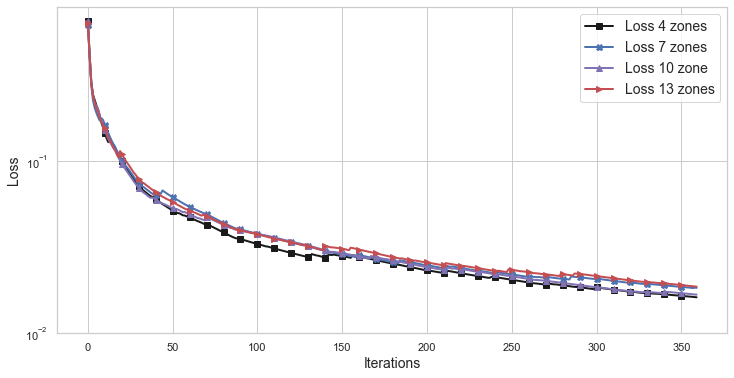
\includegraphics[width=7cm]{./img/loss6.png}
    \caption{Loss values of different network size on complete topology. \textit{(Plot on log-scale)}}
    \label{fig:loss-multiple-size}
\end{figure}


\begin{figure}
    \centering
    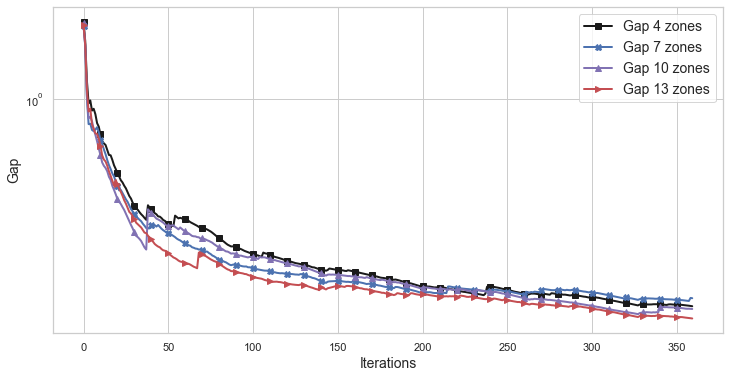
\includegraphics[width=0.45\textwidth]{./img/gap4.png}
    \caption{Gap values of different network size on complete topology.
    \textit{(Plot on log-scale)}}
    \label{fig:gap-multiple-size}
\end{figure}



\begin{table}[]
\centering
\begin{tabular}{|l|l|l|l|}
\hline
Nodes & Floors   & MSE & MAE    \\ \hline
13 & 4567   & 0.85 & 1.26  \\ \hline
10 & 456 	& 0.71 & 1.01 \\ \hline
7 & 67     & \textbf{0.65} &	\textbf{0.78} \\ \hline 
4 & 6    &	1.5 &	0.99\\ \hline
\end{tabular}
\caption{Performance comparison between 4 network configurations  }
\label{table:temp4comp}
\end{table}


% \begin{figure}%
%     \centering
%     \subfloat[\centering Floor 4 and 5   ]{{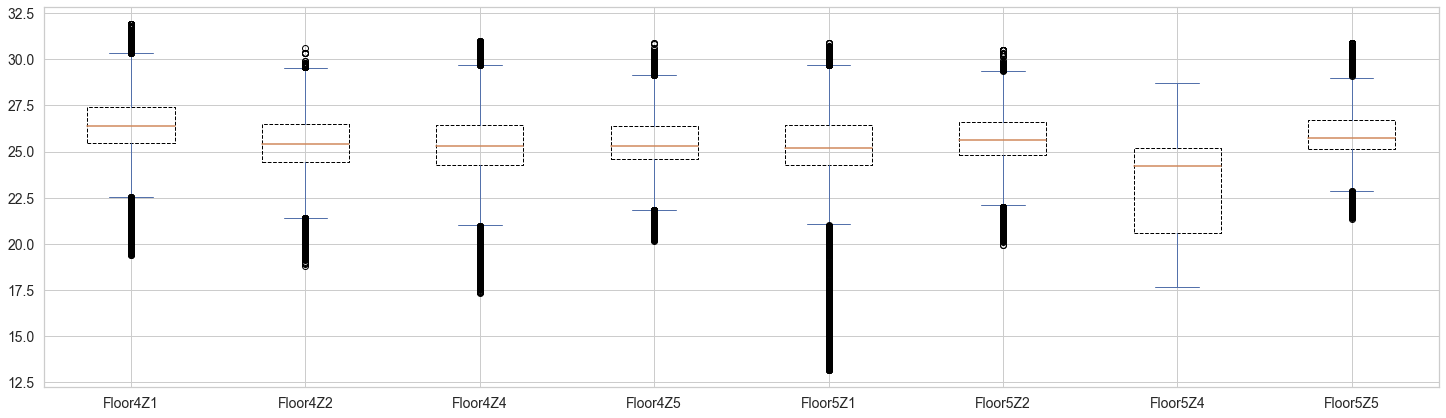
\includegraphics[width=7cm]{./img/tempVariation45.png} }}%
%     \qquad
%     \subfloat[\centering Floors 6 and 7     ]{{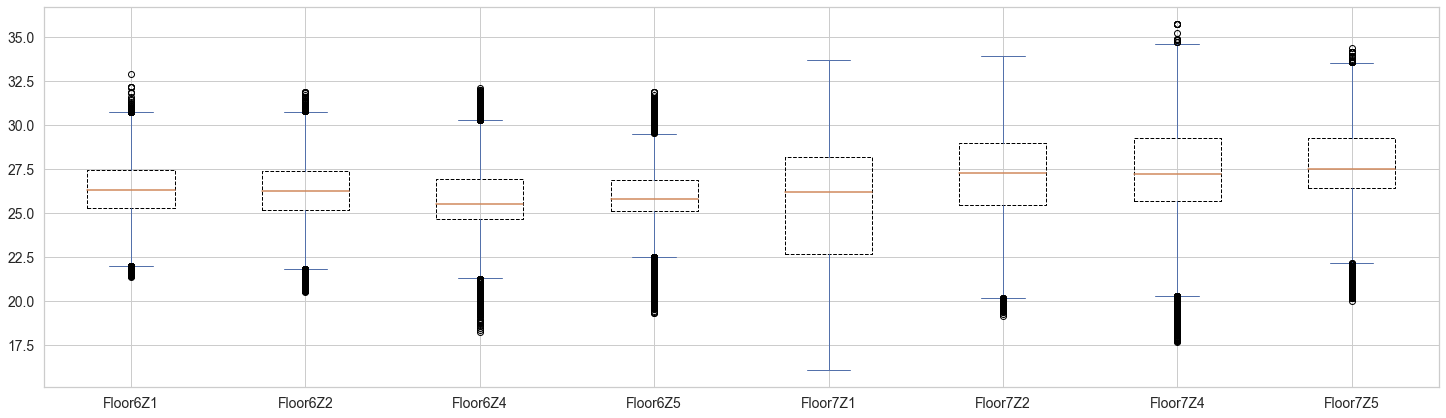
\includegraphics[width=7cm]{./img/tempVariation67.png}}}%
%     \caption{Data Distribution of Temperature for 16 zones across 4 floors}%
%     \label{fig:tempVariation}%
% \end{figure}



\subsection{Effect of Network Topology on Learning}

% Now that we have a reliable proof of effectiveness for the approach per floor, we analyze the effect of topology in a bigger consortium of co-operating learners. 
% \begin{table}[]
% \centering
% \begin{tabular}{|l|l|l|l|}
% \hline
% Nodes & \multicolumn{3}{l|}{Edges} \\ \hline
%       & Complete  & Cycle  & Line  \\ \hline
% 7     & 28        & 7      & 6     \\ \hline
% 13    & 78        & 13     & 12    \\ \hline
% \end{tabular}
% \caption{Comparison between 6 network configurations. }
% \label{tab:networkSize}
% \end{table}

We study the effect of topology in learning %through by increasing networks in terms of links or nodes. 
% The graph configuration between 6 network sizes are given in Table \ref{tab:networkSize}.
for a 7 node configuration with a complete, cycle and line graph containing 28, 7 and 6 edges respectively and with 13 nodes having 78,13 and 12 edges respectively. 
For both 7 (Table \ref{table:temp8}) and 13 (Table \ref{table:temp13}) node configurations, we observe that the complete graph yields the least amount of prediction error, mean absolute error $\in [0.66, 1.3] \degree C$. 
However we note the peculiarity that the line graph can perform better than a cycle graph and has roughly a 10 $\%$ error margin compared to the complete configuration.

\begin{comment}
 \begin{figure}[ht]
    \centering
\subfloat[][]{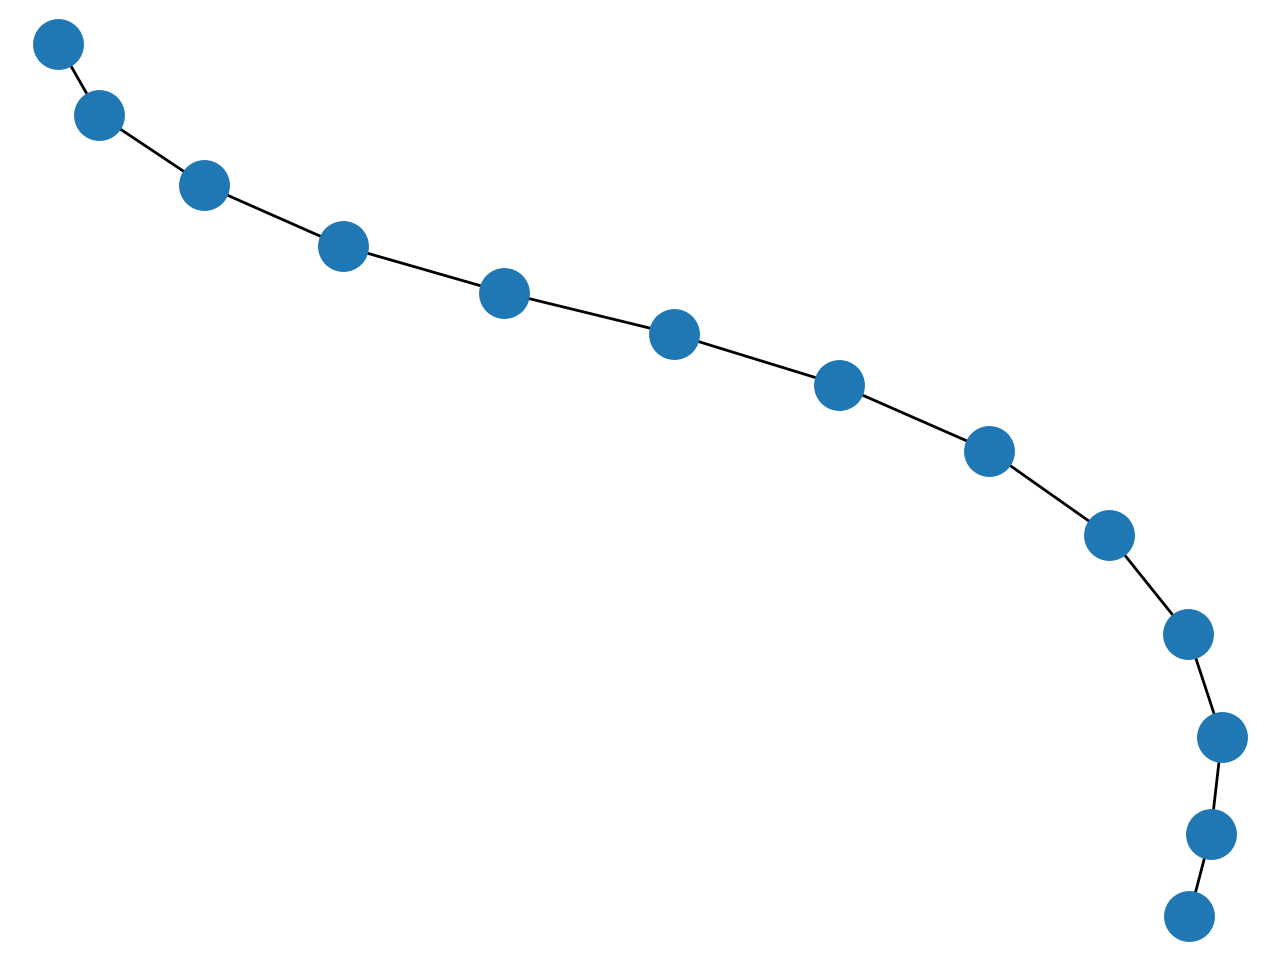
\includegraphics[width=0.16\textwidth]{./img/13L.png}} 
\subfloat[][]{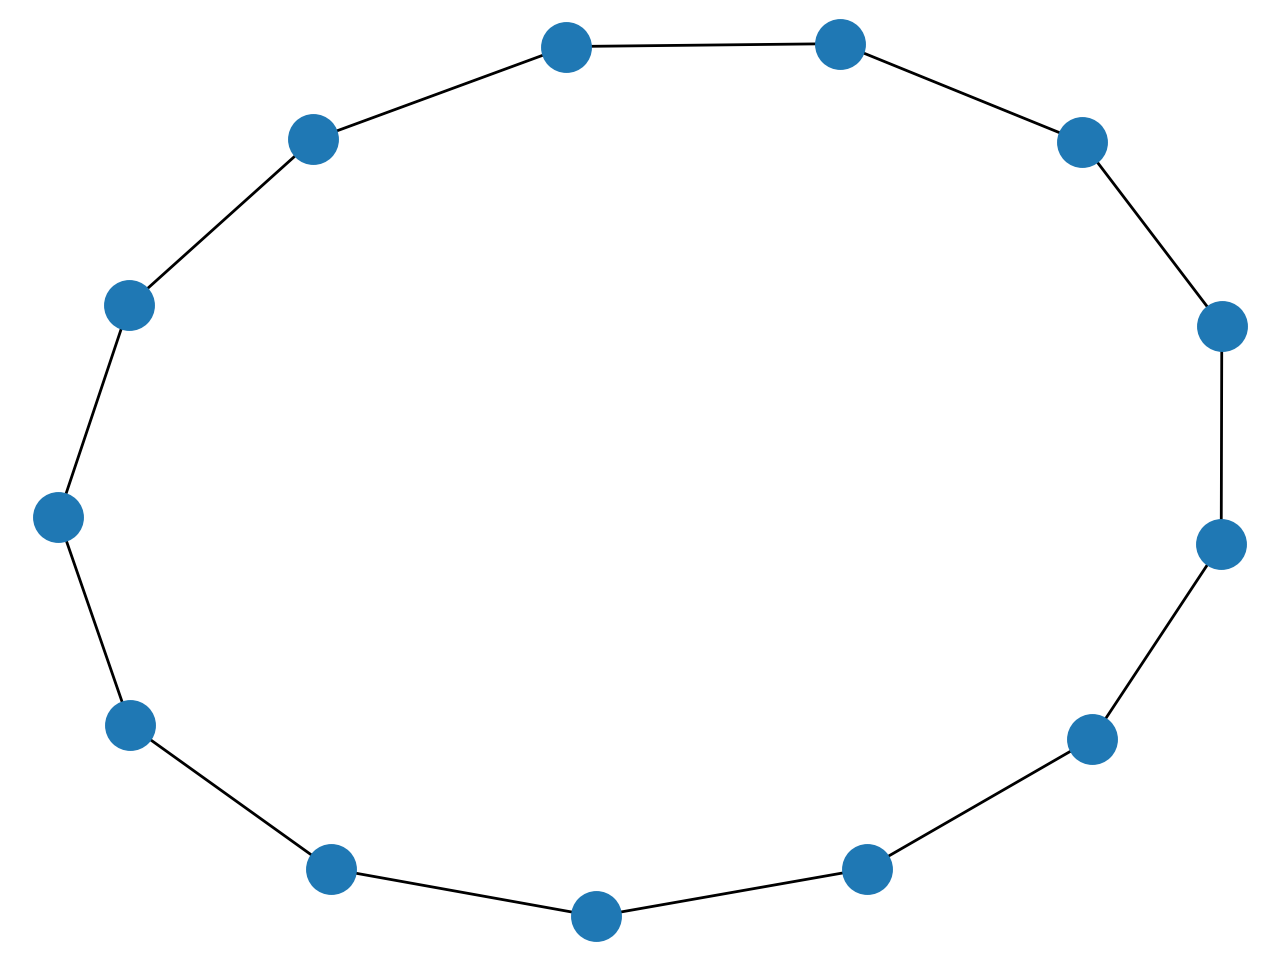
\includegraphics[width=0.16\textwidth]{./img/13N.png}}
\subfloat[][]{\includegraphics[width=0.16\textwidth]{./img/K13.png}}
    \caption{13 Node configuration}
    \label{fig:network13}%
    \end{figure}
\end{comment}


\begin{table}[]
\begin{tabular}{|l|l|l|l|l|l|}
\hline
Topology & Metric    & Mean & Variance & Max   & Min \\ \hline
cycle    & MAE   & 1.099 & 0.485  & 1.808 &  0.56 \\ \hline
cycle    & MSE  &  0.788 & 0.21  & 1.094 &  0.529  \\ \hline
complete & MAE   & \textbf{0.778} & 0.381 & 1.478 & 0.27 \\ \hline
complete & MSE  & \textbf{0.646} & 0.202 & 1.047 & 0.39 \\ \hline
line     & MAE   & 0.813 & 0.532 & 1.953 & 0.243 \\ \hline
line     & MSE   & 0.667 & 0.288 & 1.266 & 0.344 \\ \hline
\end{tabular}
\caption{Impact of Networking on 7 learners configuration. }
\label{table:temp8}
\end{table}


\begin{table}[ht]
\begin{tabular}{|l|l|l|l|l|l|}
\hline
Topology & Metric & Mean & Variance & Max   & Min   \\ \hline
cycle    & MAE   & 1.511 & 1.456 & 6.159 & 0.361 \\ \hline
cycle    & MSE   & 0.938  & 0.384  & 1.897  & 0.483 \\ \hline
complete & MAE  & \textbf{1.257 }& \textbf{0.82} & 3.64 & \textbf{0.32} \\ \hline
complete & MSE   & \textbf{0.852} & \textbf{0.272} & \textbf{1.505} & 0.417 \\ \hline
line     & MAE   & 1.385 & 0.915 & 3.169 & 0.5 \\ \hline
line     & MSE   & 0.905 & 0.352 & \textbf{1.664} & 0.492 \\ \hline
\end{tabular}
\caption{Impact of Topology on Temperature Forecasting Performance with 13 learners.}
\label{table:temp13}
\end{table}




\subsection{Effect of Decentralization}

We are interested to understand the role of decentralization in terms of accuracy of zonal learners.
Let $L_{MFW}(t)$ be the loss from Meta Frank Wolfe (MFW) at time $t$.
The approximation ratio $$A(t) = \frac{L_{DMFW}(t) }{L_{MFW}(t)}$$ at time $t$ is a heuristic to define how worse is our decentralized version compared to a centralized optimization. 
$A(t) \leq B_{max}$ will mean our algorithm performs no worse than $B_{max}$ times of the MFW.
%
Figure \ref{fig:loss_baseline} shows that our algorithm performs slightly worse than MFW. On figure \ref{fig:ratio}, we plot the ratio $A(t)$ for a 13 node network and show that $A(t) \leq 1.4$. 
The 7 node network has the closest approximation bounded by $1.35$ which can be explained by earlier insights on performance accuracy.  
We notice that that the 10 node network performs worst till $t = 200$ and after  $t \geq 250 $ or 21 hours, the approximation ratio becomes close to centralised version with less than 20 $\%$ error.


\begin{figure}
    \centering
    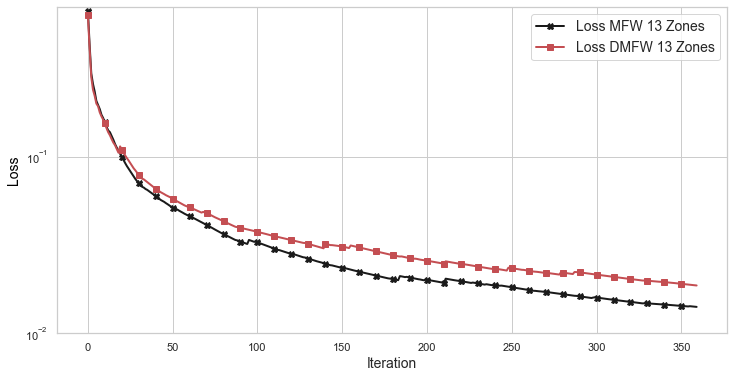
\includegraphics[width=7cm]{./img/baseline-compare/loss5.png}
    \caption{Loss values of decentralized and centralized Meta Frank-Wolfe \textit{(Plot on log-scale)}. We use data from 13 zones connected over a complete topology on decentralized setting \textit{(red curve)} to compare with its centralized counterpart \textit{(black curve)}}
    \label{fig:loss_baseline}
\end{figure}

\begin{figure}
    \centering
    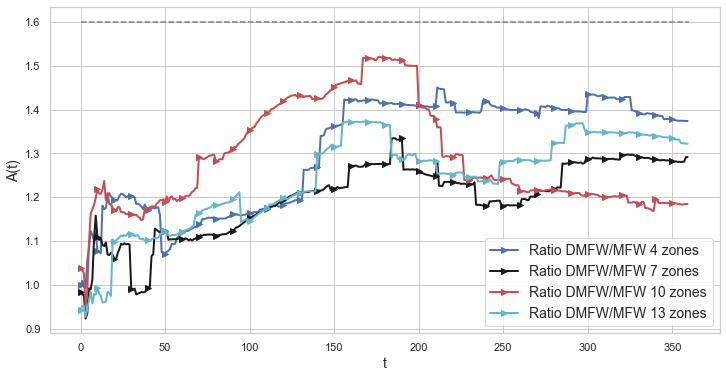
\includegraphics[width=7cm]{./img/baseline-compare/ratio_multiple_setting.png}
    \caption{Loss ratio of decentralized and centralized Meta Frank-Wolfe on different network size.}
    \label{fig:ratio}
\end{figure}


% =======================ROUGHWORK================================
% \begin{table}[]
% \centering
% \begin{tabular}{|l|l|l|l|l|}
% \hline
% \textbf{Temperature }      & Floor 3 & Floor 4 & Floor 5 & Floor 7 \\ \hline
% Line &   0.026  &   0.030    &   0.037   &   0.022   \\ \hline
% Cycle    & 0.029    &   0.030   &  0.030    &     0.027  \\ \hline
% Complete & 0.162    &   0.159   &   0.165   &    0.148   \\ \hline
% \end{tabular}
% \qquad
% \begin{tabular}{|l|l|l|l|l|}
% \hline
% \textbf{AC Power }     & Floor 3 & Floor 4 & Floor 5 & Floor 7 \\ \hline
% Line &   0.035 &    0.040   &     0.033   &   0.043  \\ \hline
% Cycle    & 0.036  &   0.035   &    0.035   &    0.038     \\ \hline
% Complete &   0.022  &   0.025   &    0.018   &   0.022  \\ \hline
% \end{tabular}

% \end{table}


%  \begin{figure}[ht]
%     \centering
% \subfloat[][]{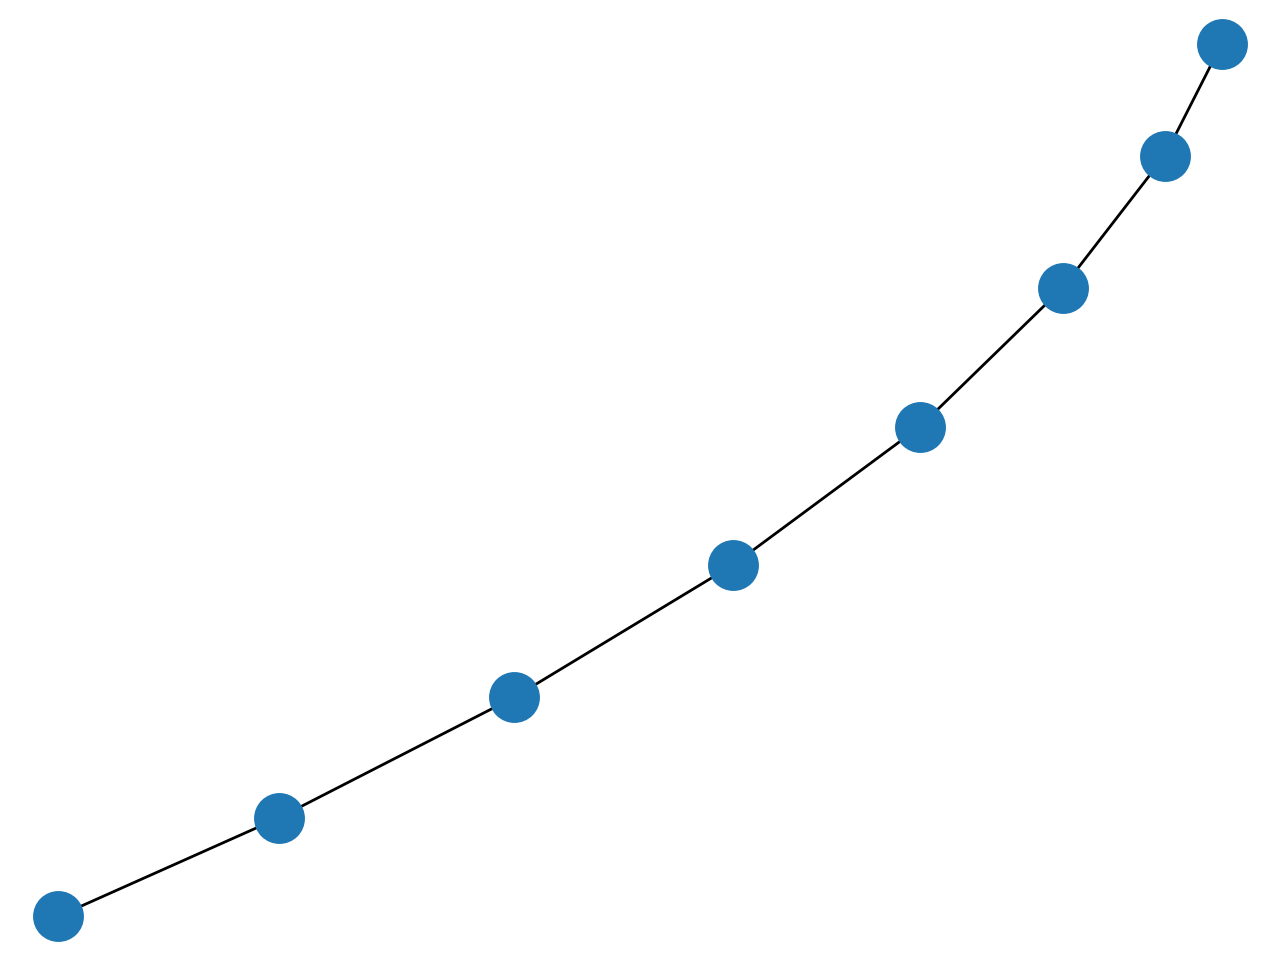
\includegraphics[width=0.16\textwidth]{img/8L.png}} 
% \subfloat[][]{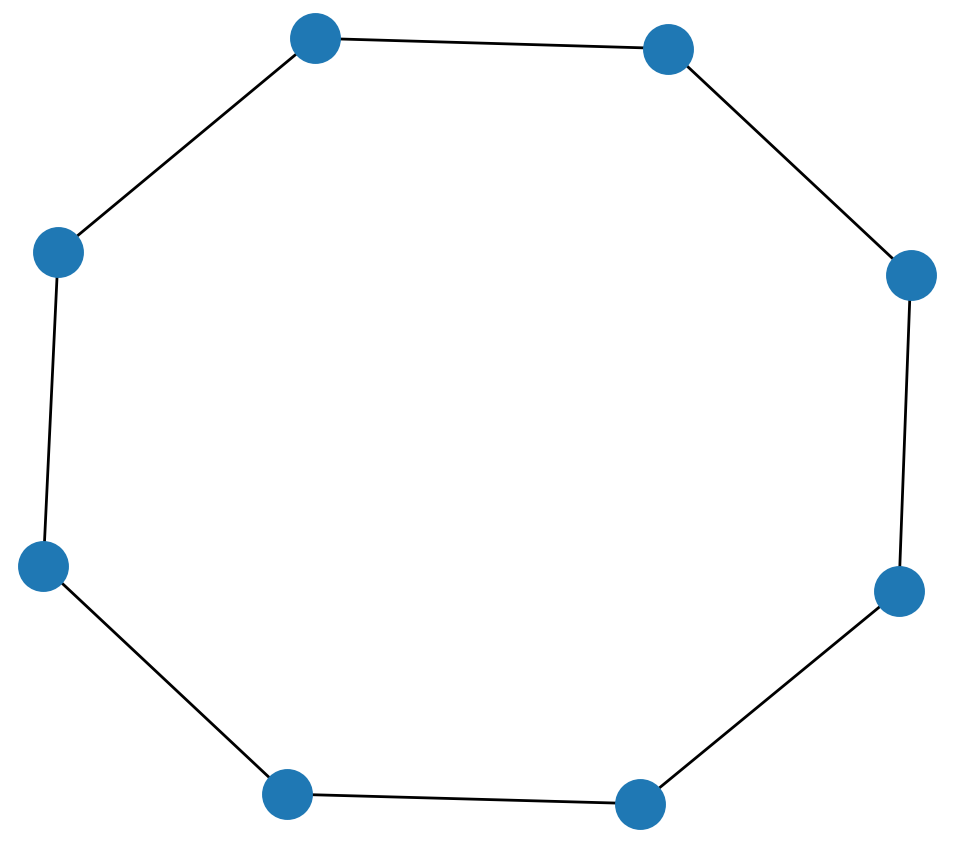
\includegraphics[width=0.16\textwidth]{img/8N.png}}
% \subfloat[][]{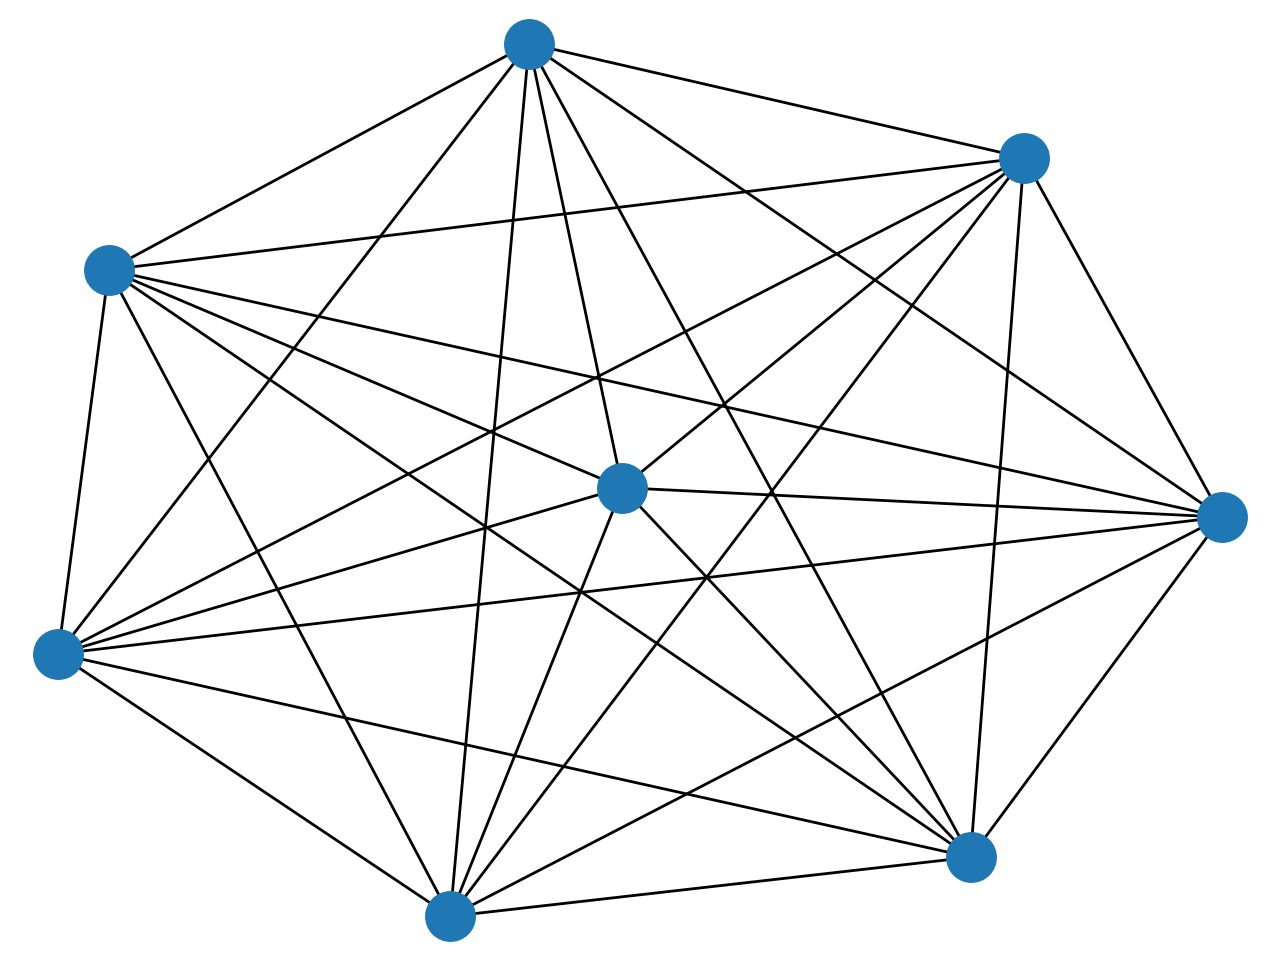
\includegraphics[width=0.16\textwidth]{img/K8.png}}
%     \caption{8 Node Network Topology}
%     \label{fig:network8}%
%     \end{figure}

% We use Online Frank-Wolfe (OFW) as benchmarks for our result. As OFW is an online centralized algorithm, we train a zone-wise model with the same training procedure as our algorithm and average the results. 





% \begin{figure}%
%     \centering
%     \subfloat[\centering Complete ]{{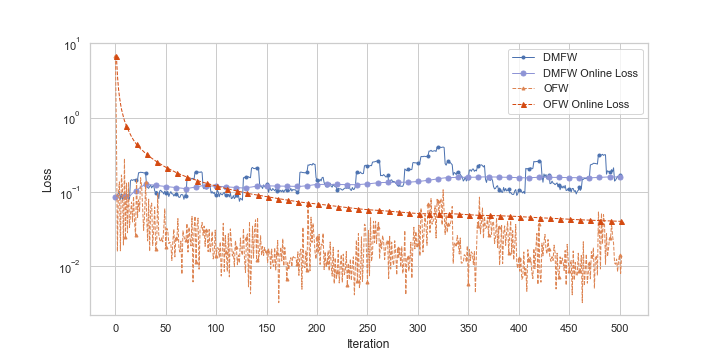
\includegraphics[width=7cm]{img/ofw_img/temp/Floor4-loss-complete-Full-False.png} }}%
%     \qquad
%     \subfloat[\centering Cycle ]{{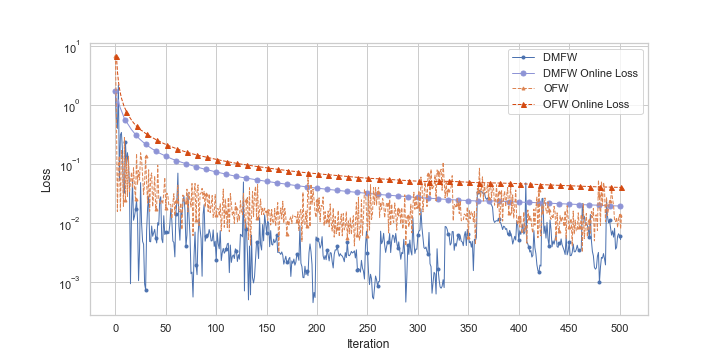
\includegraphics[width=7cm]{img/ofw_img/temp/Floor4-loss-cycle-Full-False.png} }}
%     \qquad
%     \subfloat[\centering Line ]{{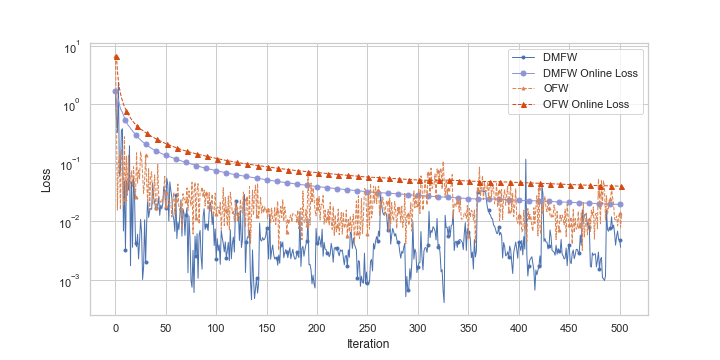
\includegraphics[width=7cm]{img/ofw_img/temp/Floor4-loss-line-Full-False.png} }}%
%     \caption{Loss value of DMFW and OFW for temperature prediction with different network connection}%
%     \label{fig:f5z4}%
% \end{figure}

% \begin{figure}%
%     \centering
%     \subfloat[\centering Complete ]{{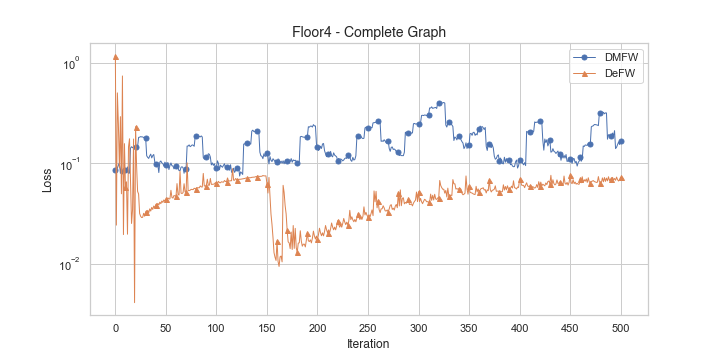
\includegraphics[width=7cm]{img/Floor4-Complete.png} }}%
%     \qquad
%     \subfloat[\centering Cycle ]{{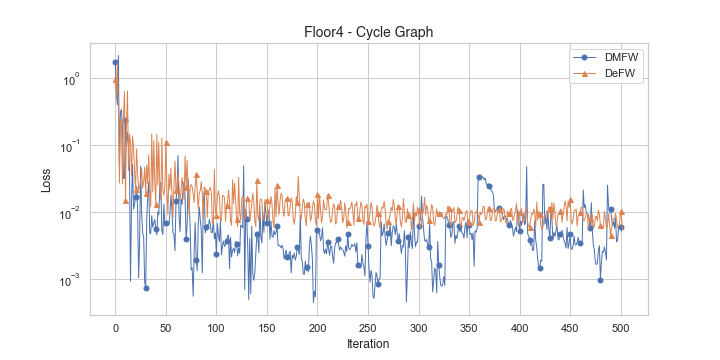
\includegraphics[width=7cm]{img/Floor4-Cycle.png} }}
%     \qquad
%     \subfloat[\centering Line ]{{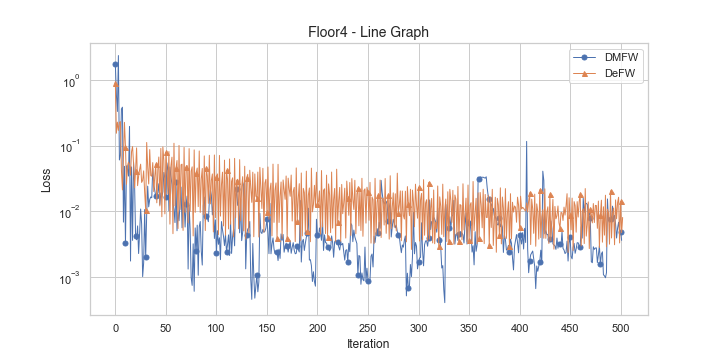
\includegraphics[width=7cm]{img/Floor4-Line.png} }}%
%     \caption{Loss value of DMFW and DeFW for temperature prediction with different network connection}%
%     \label{fig:f5z4}%
% \end{figure}


% \begin{table}[]
% \centering
% \begin{tabular}{|l|l|l|l|l|}
% \hline
% Floor 2 & Floor 3 & Floor 5 & Floor 7 \\ \hline
%  0.07 $\pm$   0.06    &   0.07 $\pm$   0.06 & 0.08 $\pm$  0.07  &     0.07 $\pm$ 0.05\\ \hline
% \end{tabular}\caption{Temperature}
% \label{table:tempLoss}
% \begin{tabular}{|l|l|l|l|l|}
% \hline
%  Floor 2 & Floor 3 & Floor 5 & Floor 7 \\ \hline
%  0.05 $\pm$ 0.01 &  0.05 $\pm$ 0.01  &   0.05 $\pm$ 0.03   & 0.07 $\pm$   0.02 \\ \hline
% \end{tabular}
% \caption{Luminosity}
% \label{table:luminosityLoss}
% \begin{tabular}{|l|l|l|l|l|}
% \hline
%  Floor 2 & Floor 3 & Floor 5 & Floor 7 \\ \hline
%  0.03 $\pm$ 0.01  &   0.03 $\pm$ 0.01    &  0.02 $\pm$ 0.01  &  0.03 $\pm$ 0.01  \\ \hline
% \end{tabular}
% \caption{Light Power}
% \label{table:lightPowerLoss}
% \begin{tabular}{|l|l|l|l|l|}
% \hline
%  Floor 2 & Floor 3 & Floor 5 & Floor 7 \\ \hline
% 0.03 $\pm$ 0.01   &    0.03 $\pm$ 0.01  &   0.03 $\pm$ 0.01   &  0.04 $\pm$ 0.02  \\ \hline
% \end{tabular}
% \caption{AC Power }
% \label{table:acPowerLoss}
% \end{table}
% \begin{figure}%
%     \centering
%     \subfloat[\centering Converging Gap  ]{{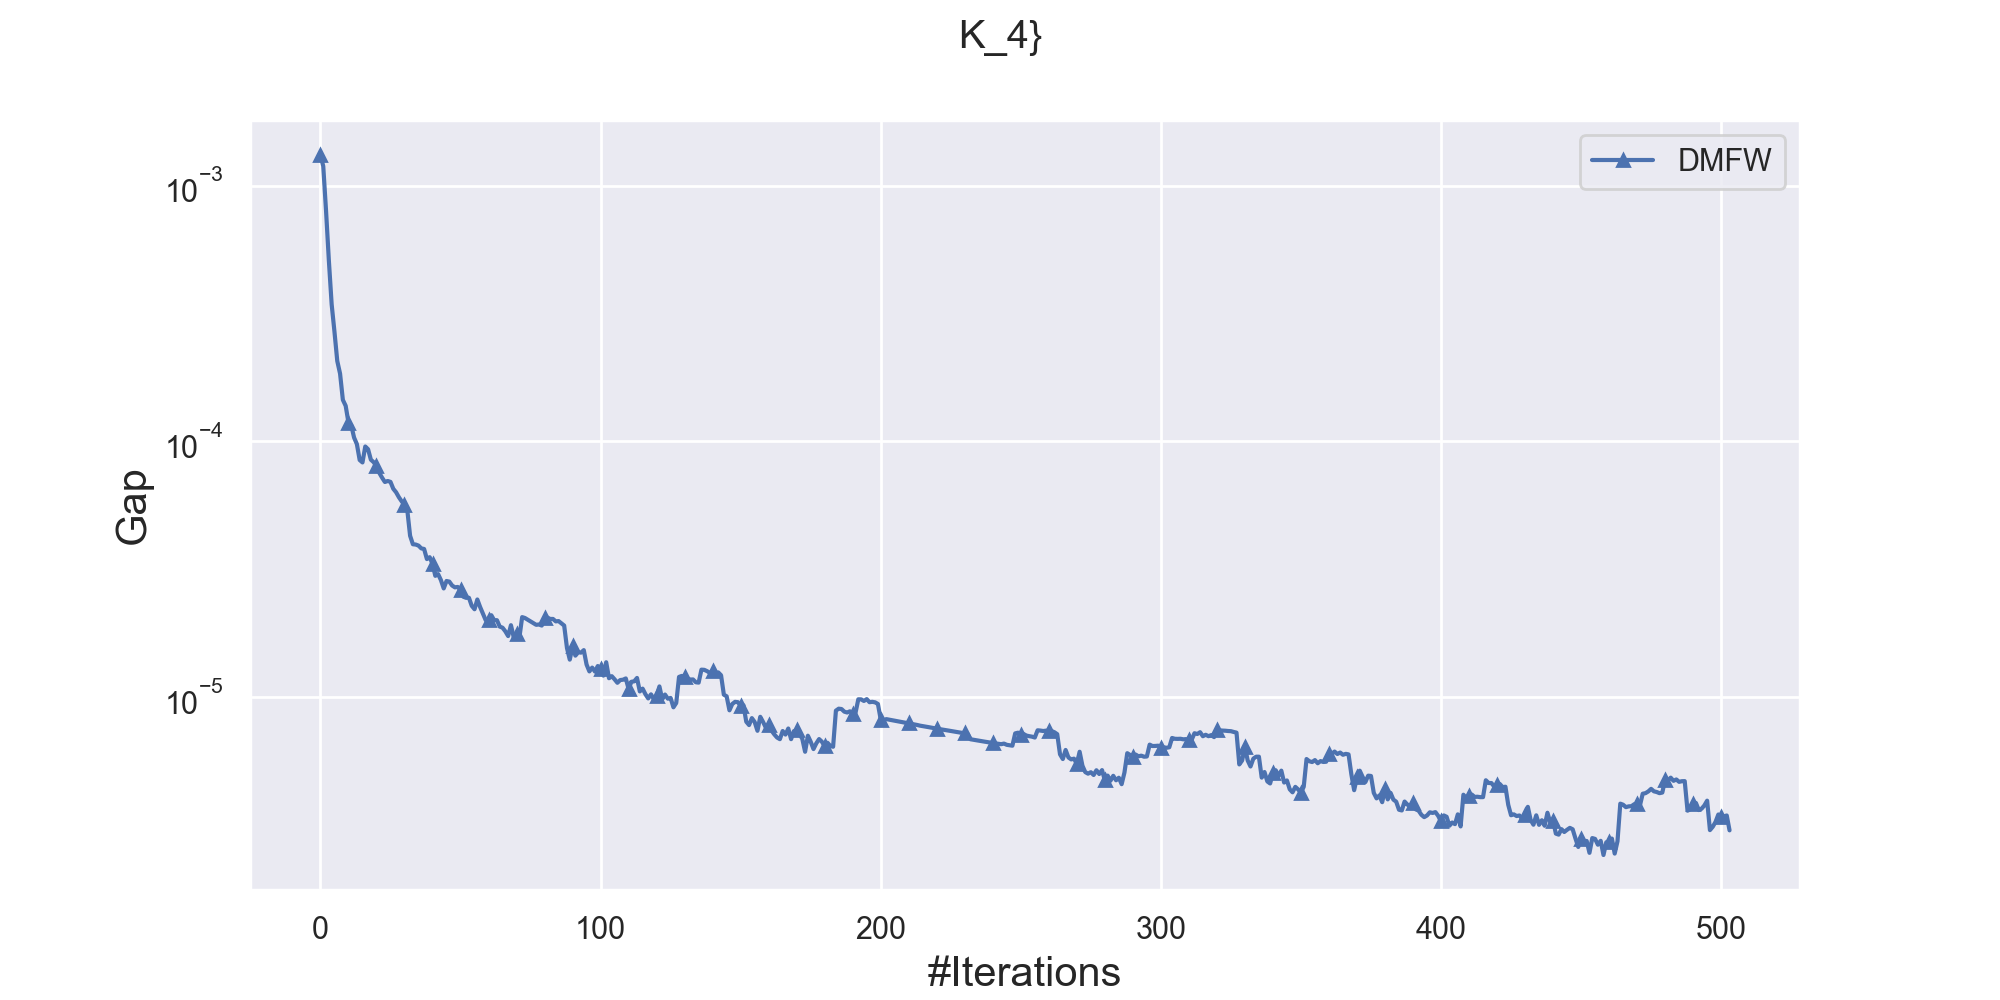
\includegraphics[width=7cm]{img/Gap-F3Z4.png} }}%
%     \qquad
%     \subfloat[\centering Oscillating Loss ]{{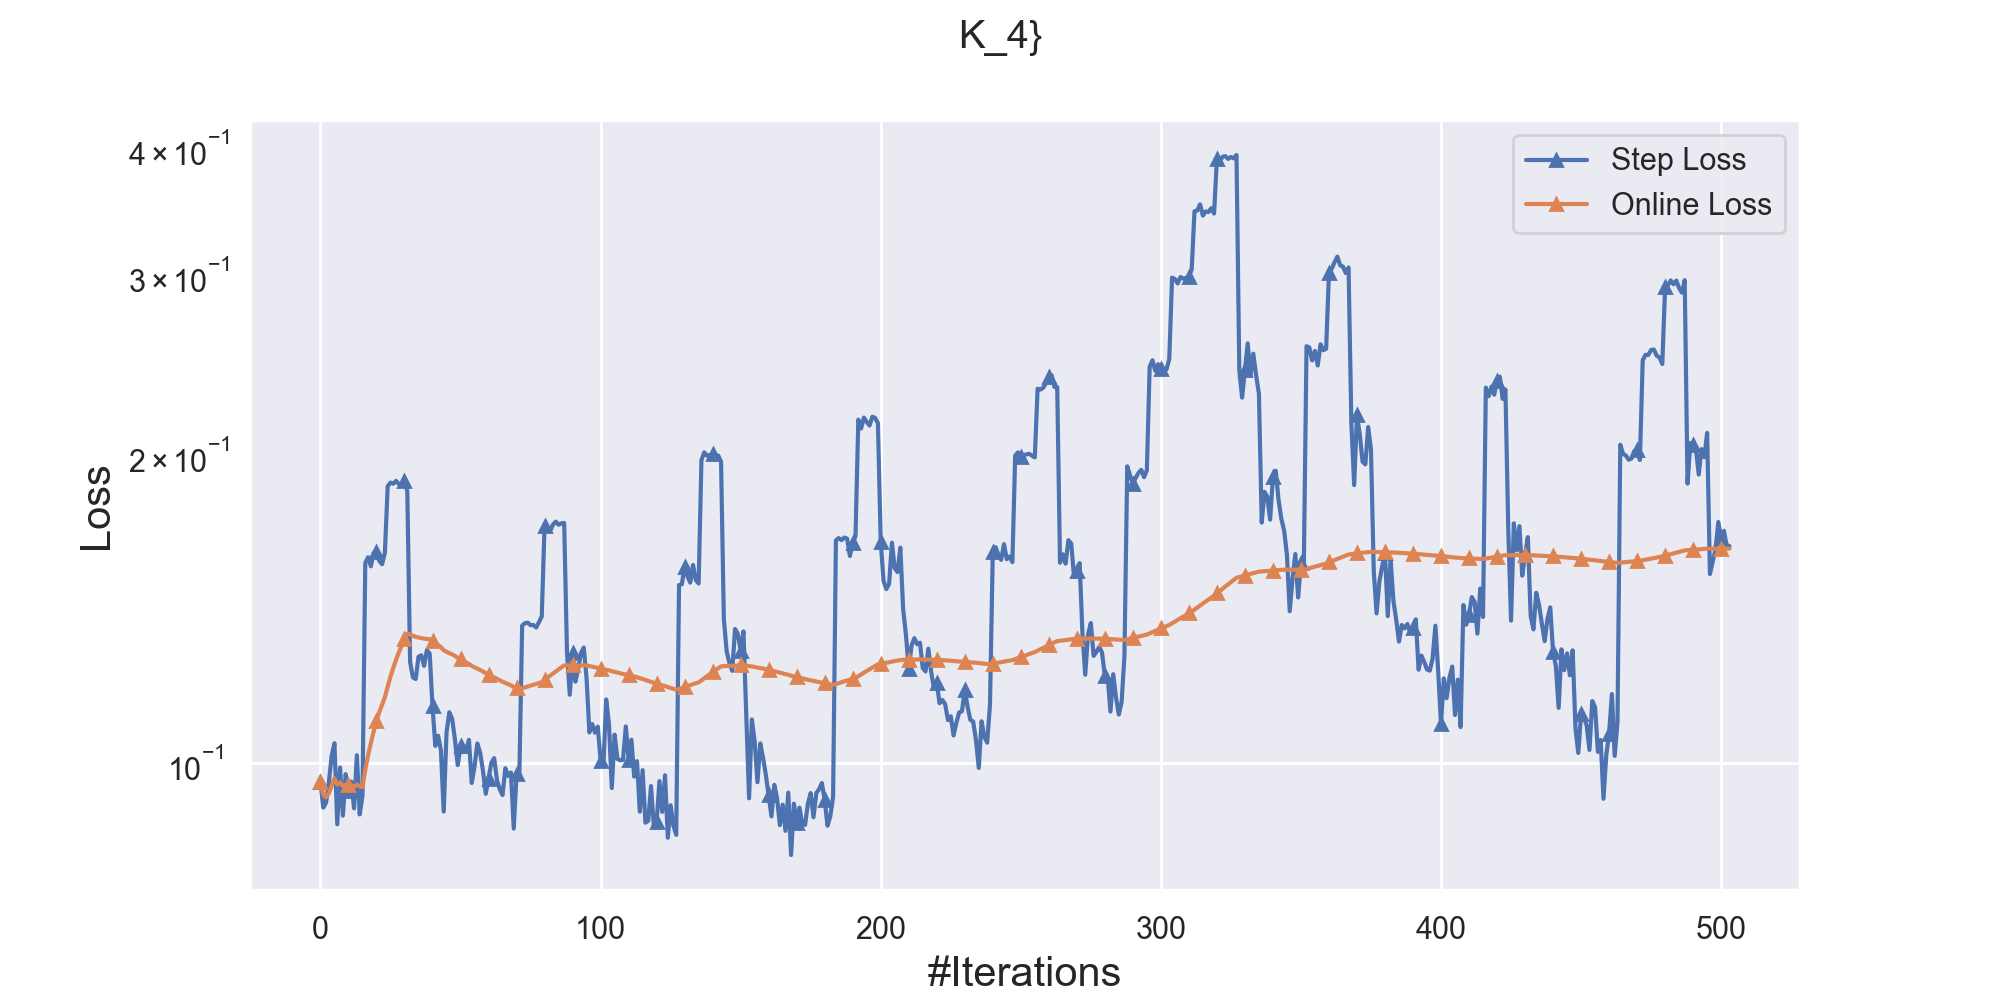
\includegraphics[width=7cm]{img/OnlineLoss-F3Z4.png} }}%
%     \caption{Evaluation metrics for a non-performing zonal model with \textbf{fully connected} network transfer. }%
%     \label{fig:f3z4}%
% \end{figure}

% \begin{figure}%
%     \centering
%     \subfloat[\centering Converging Gap  ]{{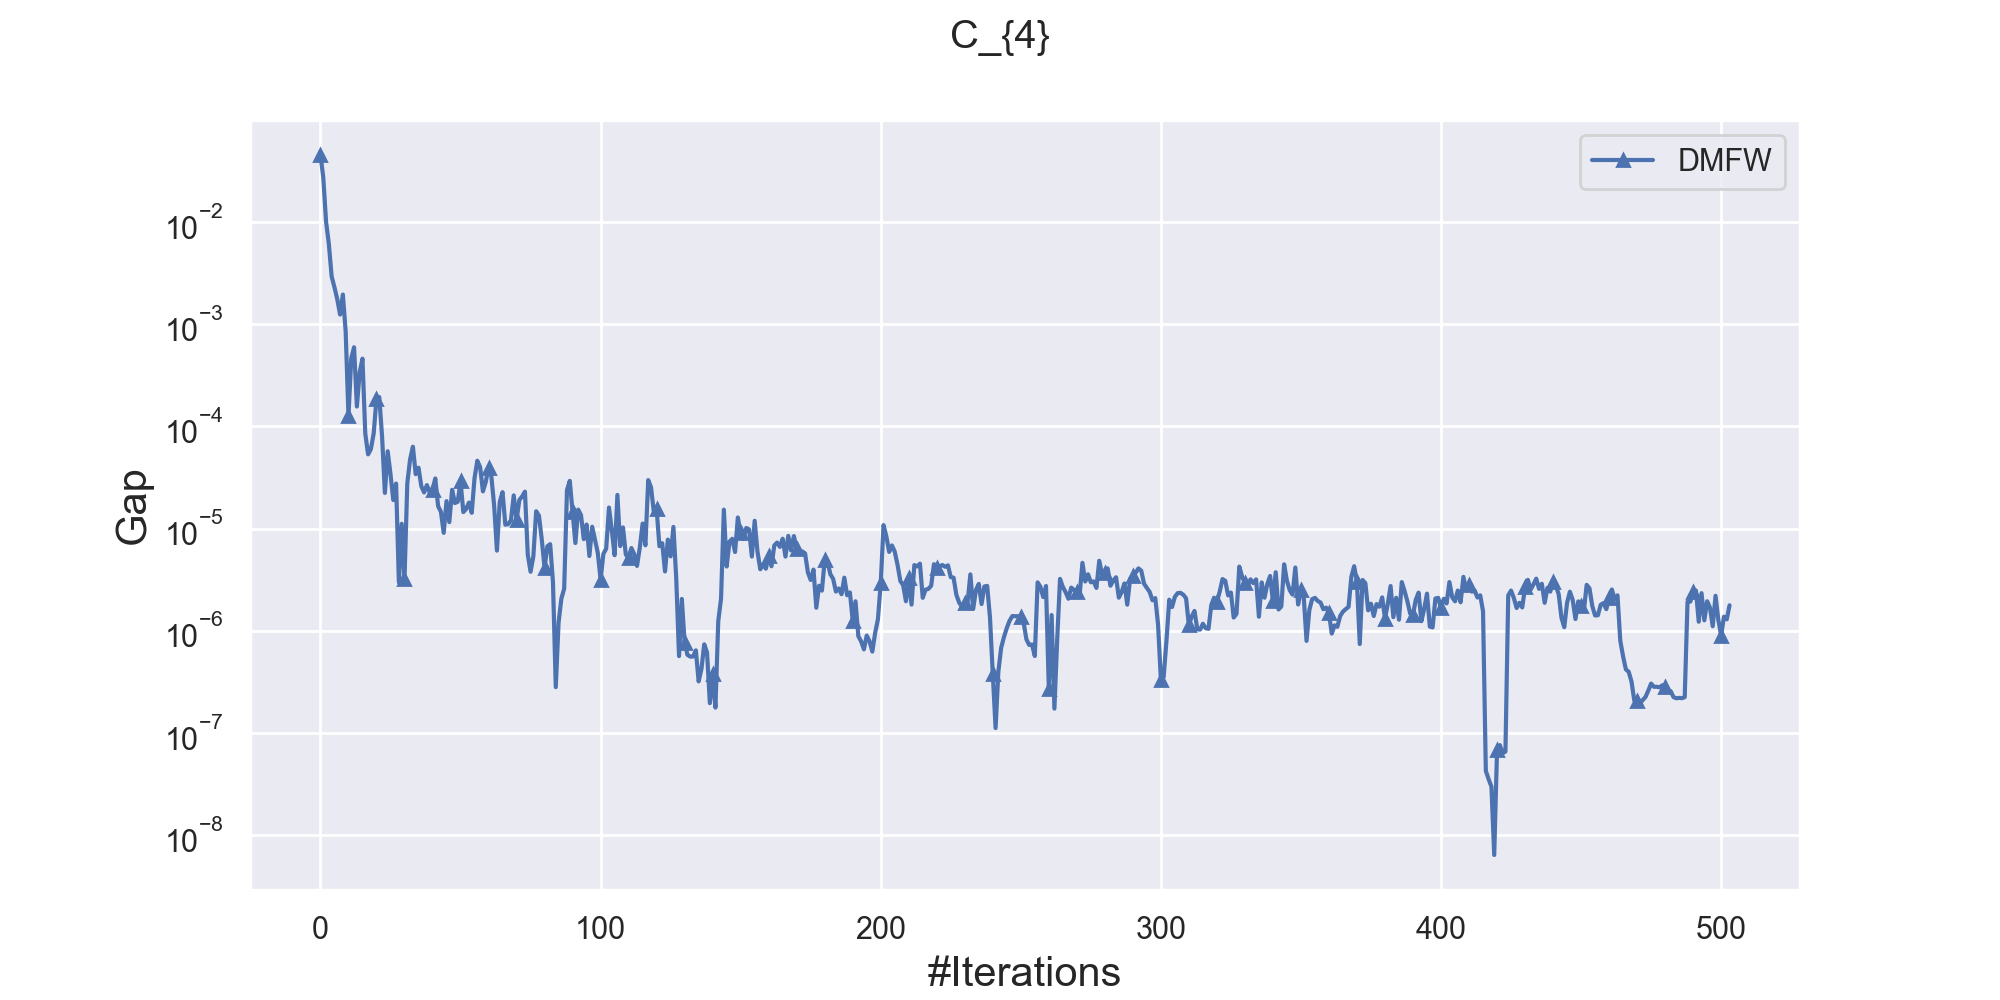
\includegraphics[width=7cm]{img/Gap-F5Z4.png} }}%
%     \qquad
%     \subfloat[\centering Decreasing Loss ]{{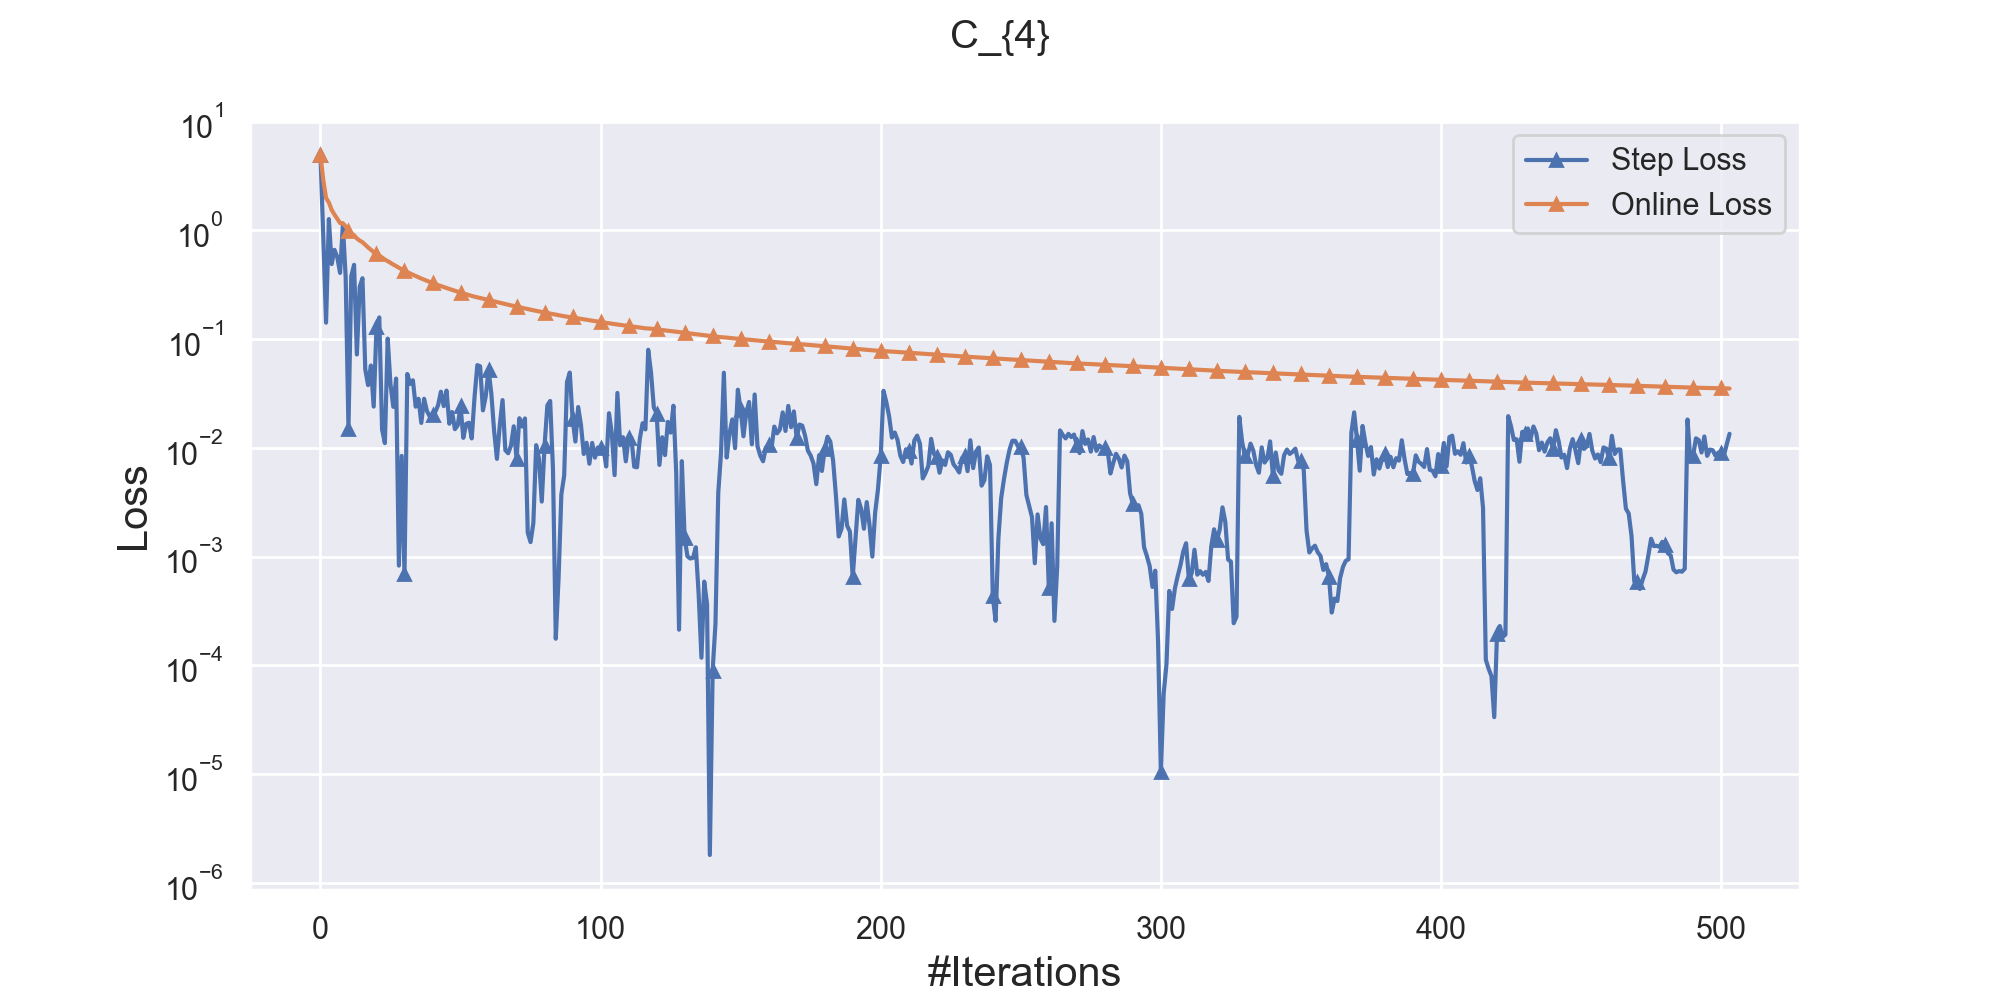
\includegraphics[width=7cm]{img/OnlineLoss-F5Z4.png} }}%
%     \caption{Evaluation metrics for a reliable zonal model with \textbf{cyclic} network connection.  }%
%     \label{fig:f5z4}%
% \end{figure}

% For a line, cycle and complete graphs with 7 and 13 nodes as shown in .

% Recall that for a line graph, every intermediate node has 2 connected neighbours except the first and last node. 
% We extend to a cyclic configuration by adding an edge between the first and last node of a line graph.
% Now every node has exactly 2 adjacent neighbours unlike a complete graph of k-1 degree.

% \begin{comment}
% Figure \ref{fig:onlineLossFloorWise} shows the prediction performance of 4 zones in floor 7 and gives a comparative study between 4 floors.
% We explain the loss for floor 4 is higher than the other floors due to dissimilar patterns from zones in that floor.
% Tables \ref{table:tempLoss}, \ref{table:luminosityLoss}, \ref{table:luxPowerNetwork}, \ref{table:acPowerLoss} record the average loss of 4 zonal models per floor for forecasting a specified sensor channel.
% Distance of an online model at time $t$ from the optimal model at hindsight is evaluated by the gap.
% Figure \ref{fig:lossGap} shows the evolution of the gap for \textit{floor 4} and shows a comparative plot between 4 networks.
% From Table \ref{table:temp4comp}, it is evident that floor 5 has the largest error margin of around $7.7 \degree$. 
% From the box plots in Figure \ref{fig:tempVariation}, we see that the data of floor 5 has a different larger spread and behave unlike the other zone. 
% \end{comment}






% \begin{figure}%
%     \centering
%     \subfloat[\centering Instantaneous and Time Averaged Online Loss  ]{{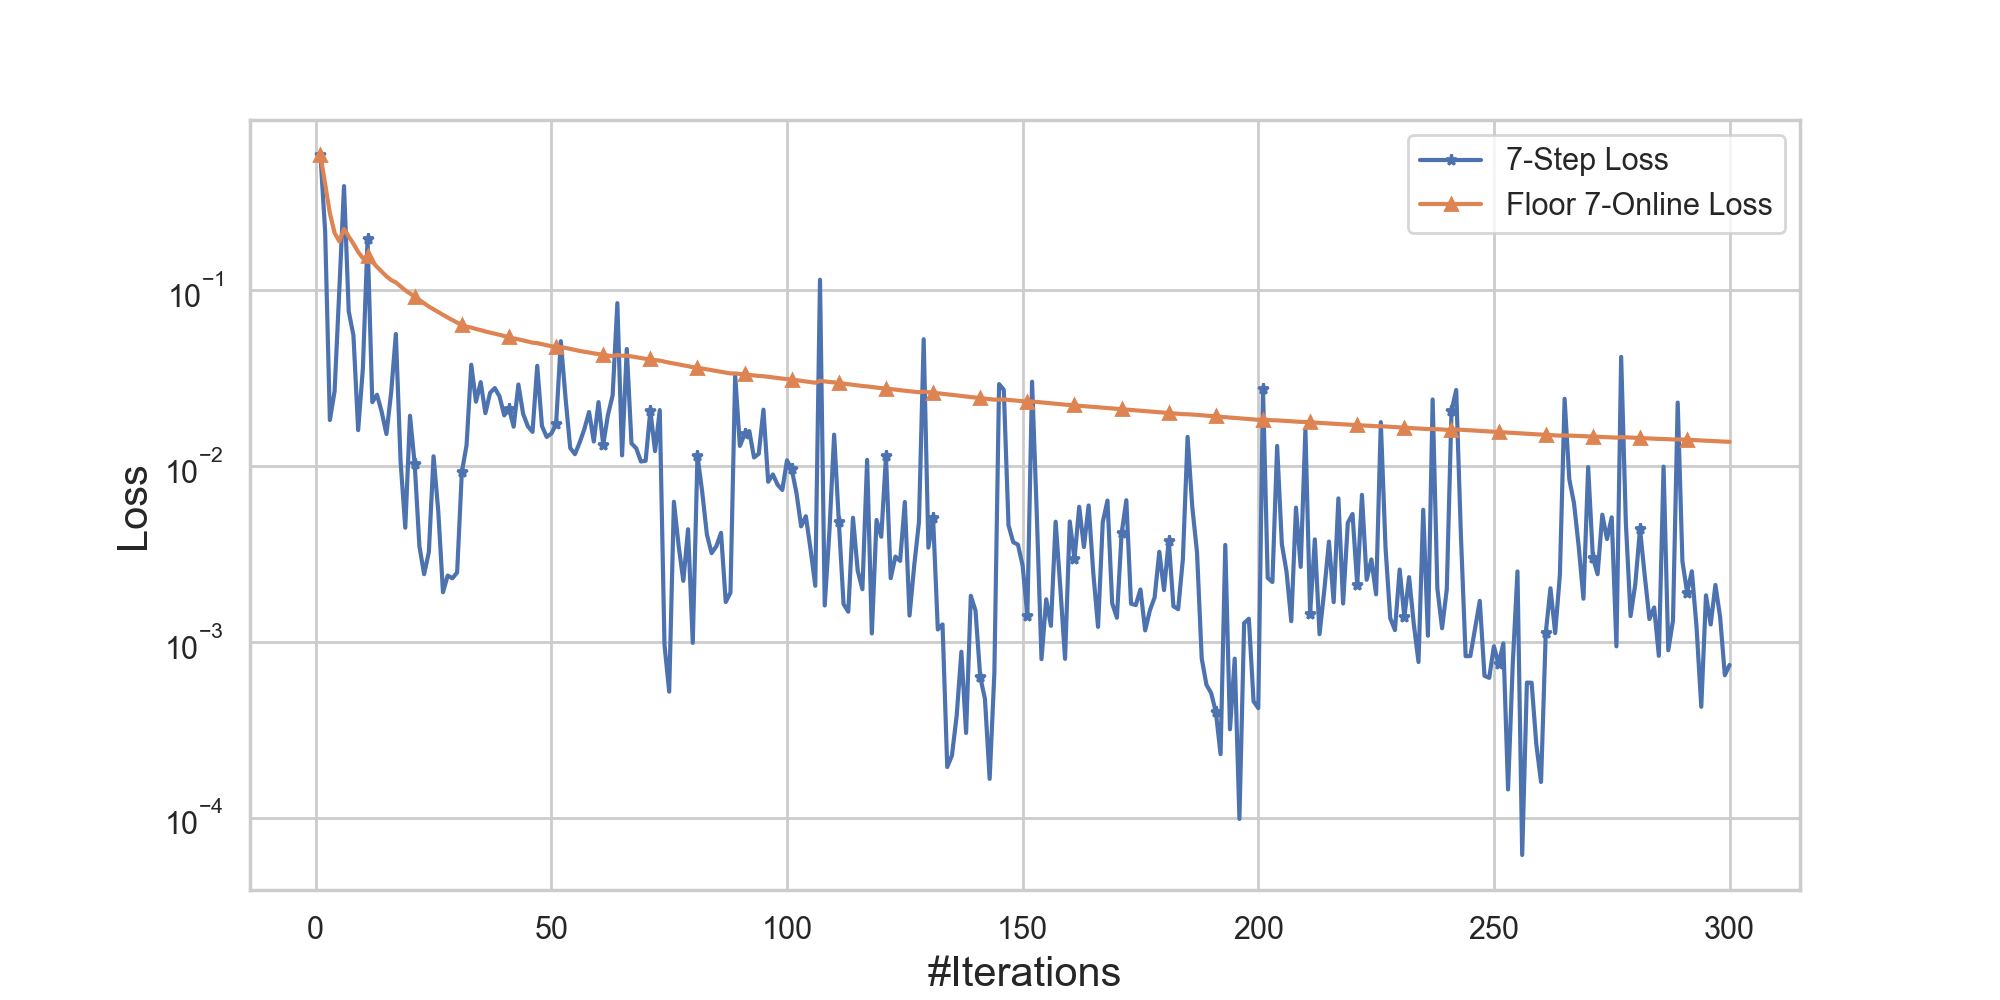
\includegraphics[width=7cm]{img/onlineLoss-f7.png} }}%
%     \qquad
    % \subfloat[\centering Comparative Floor Wise Online Losses   ]{{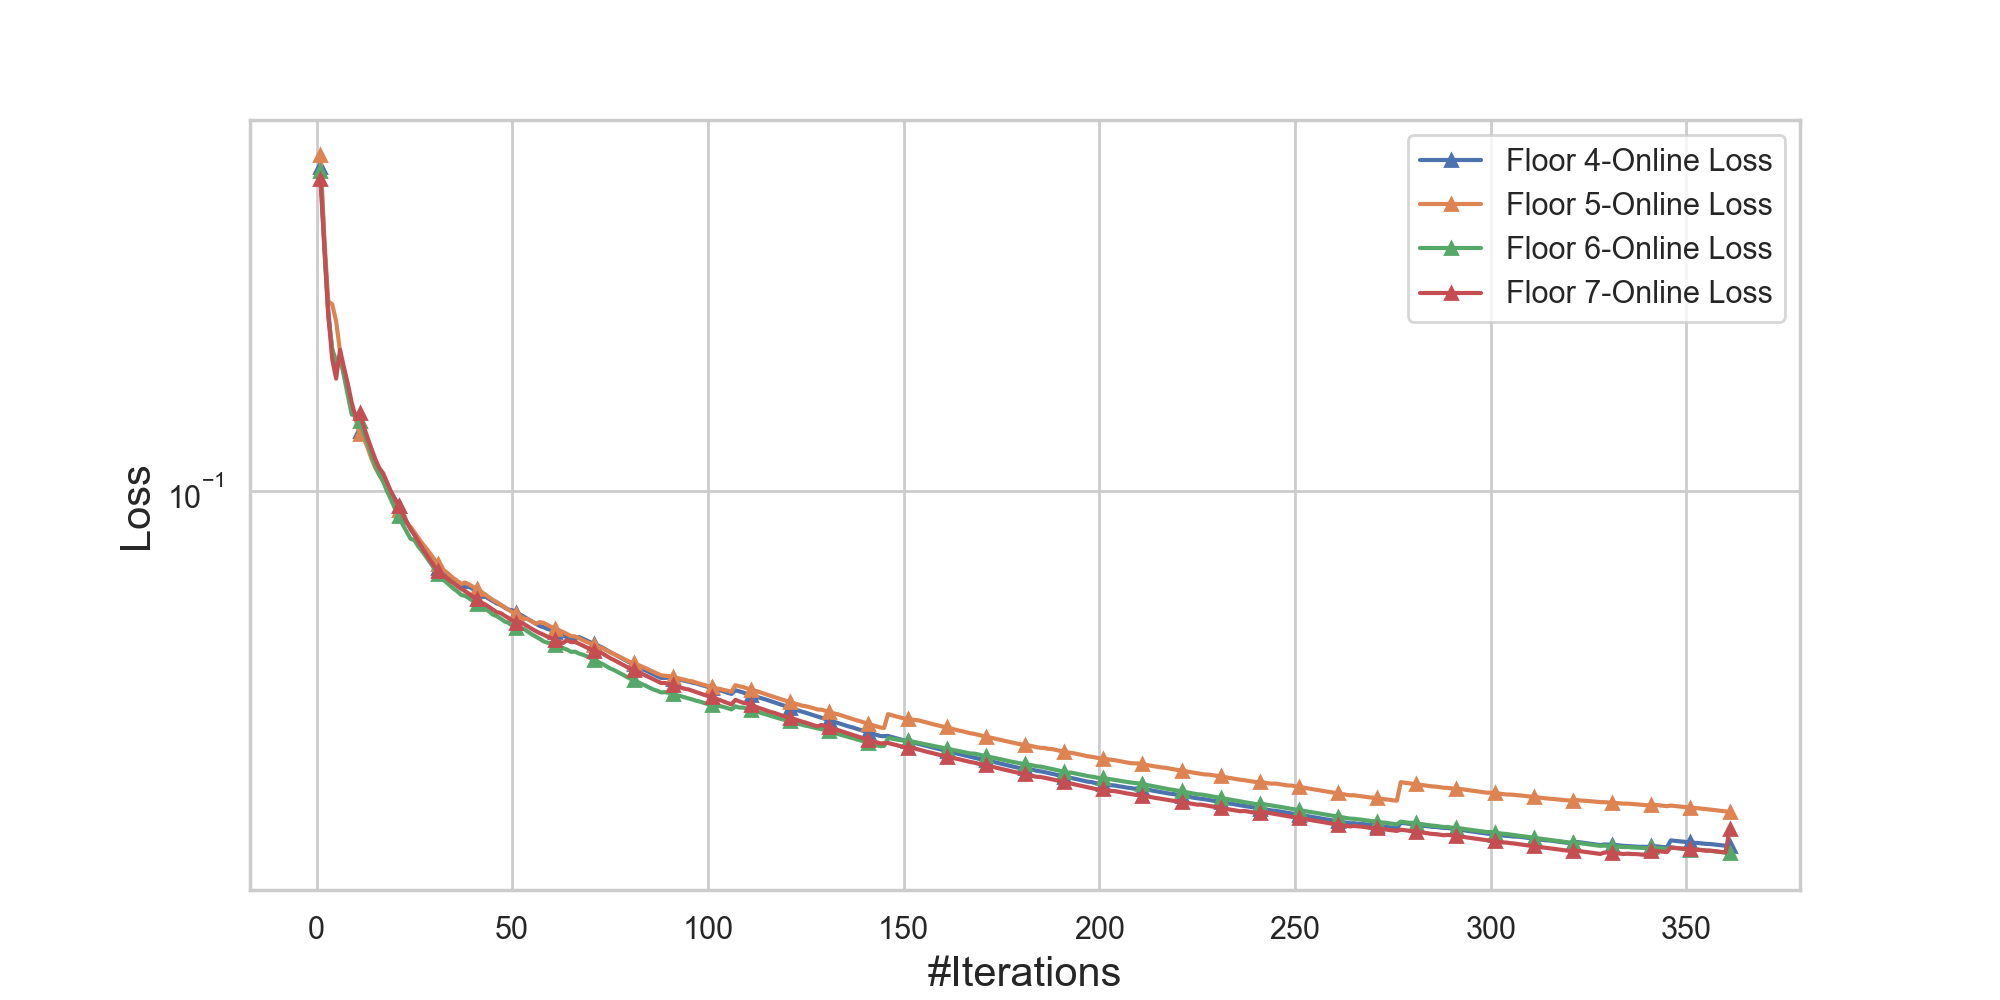
\includegraphics[width=7cm]{img/floorComp.png}}}%
%     \caption{Online Forecasting Model Performance on Indoor Zonal Temperature}%
%     \label{fig:onlineLossFloorWise}%
% \end{figure}


% \begin{figure}
%     \centering
%     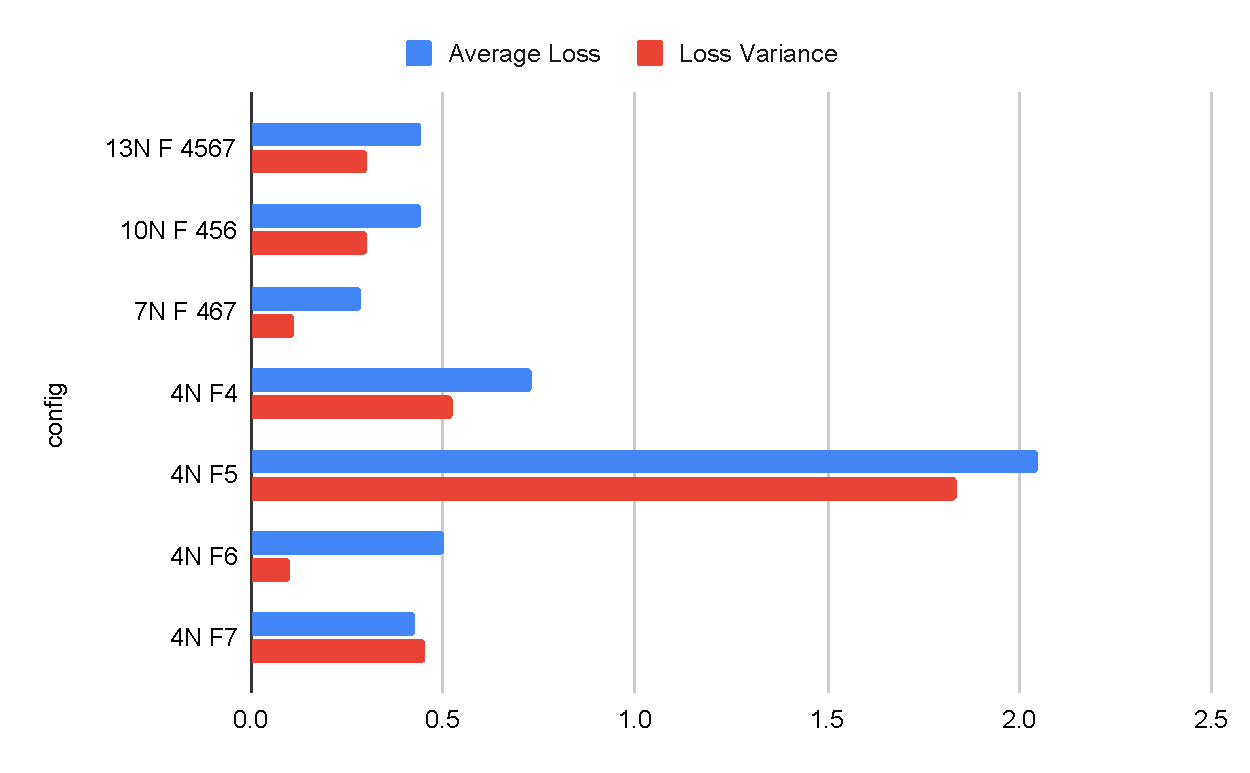
\includegraphics[width=0.5\textwidth]{img/accuracyCoverage.pdf}
%     \caption{RMSE values for 7 different learner configurations represented by $x$\textit{N} nodes from \textit{F}$i,j,k$ participating floors.}
%     \label{fig:accuracyCoverage}
% \end{figure}



% \begin{figure}%
%     \centering
%     \subfloat[\centering Gaps and Local Gaps  ]{{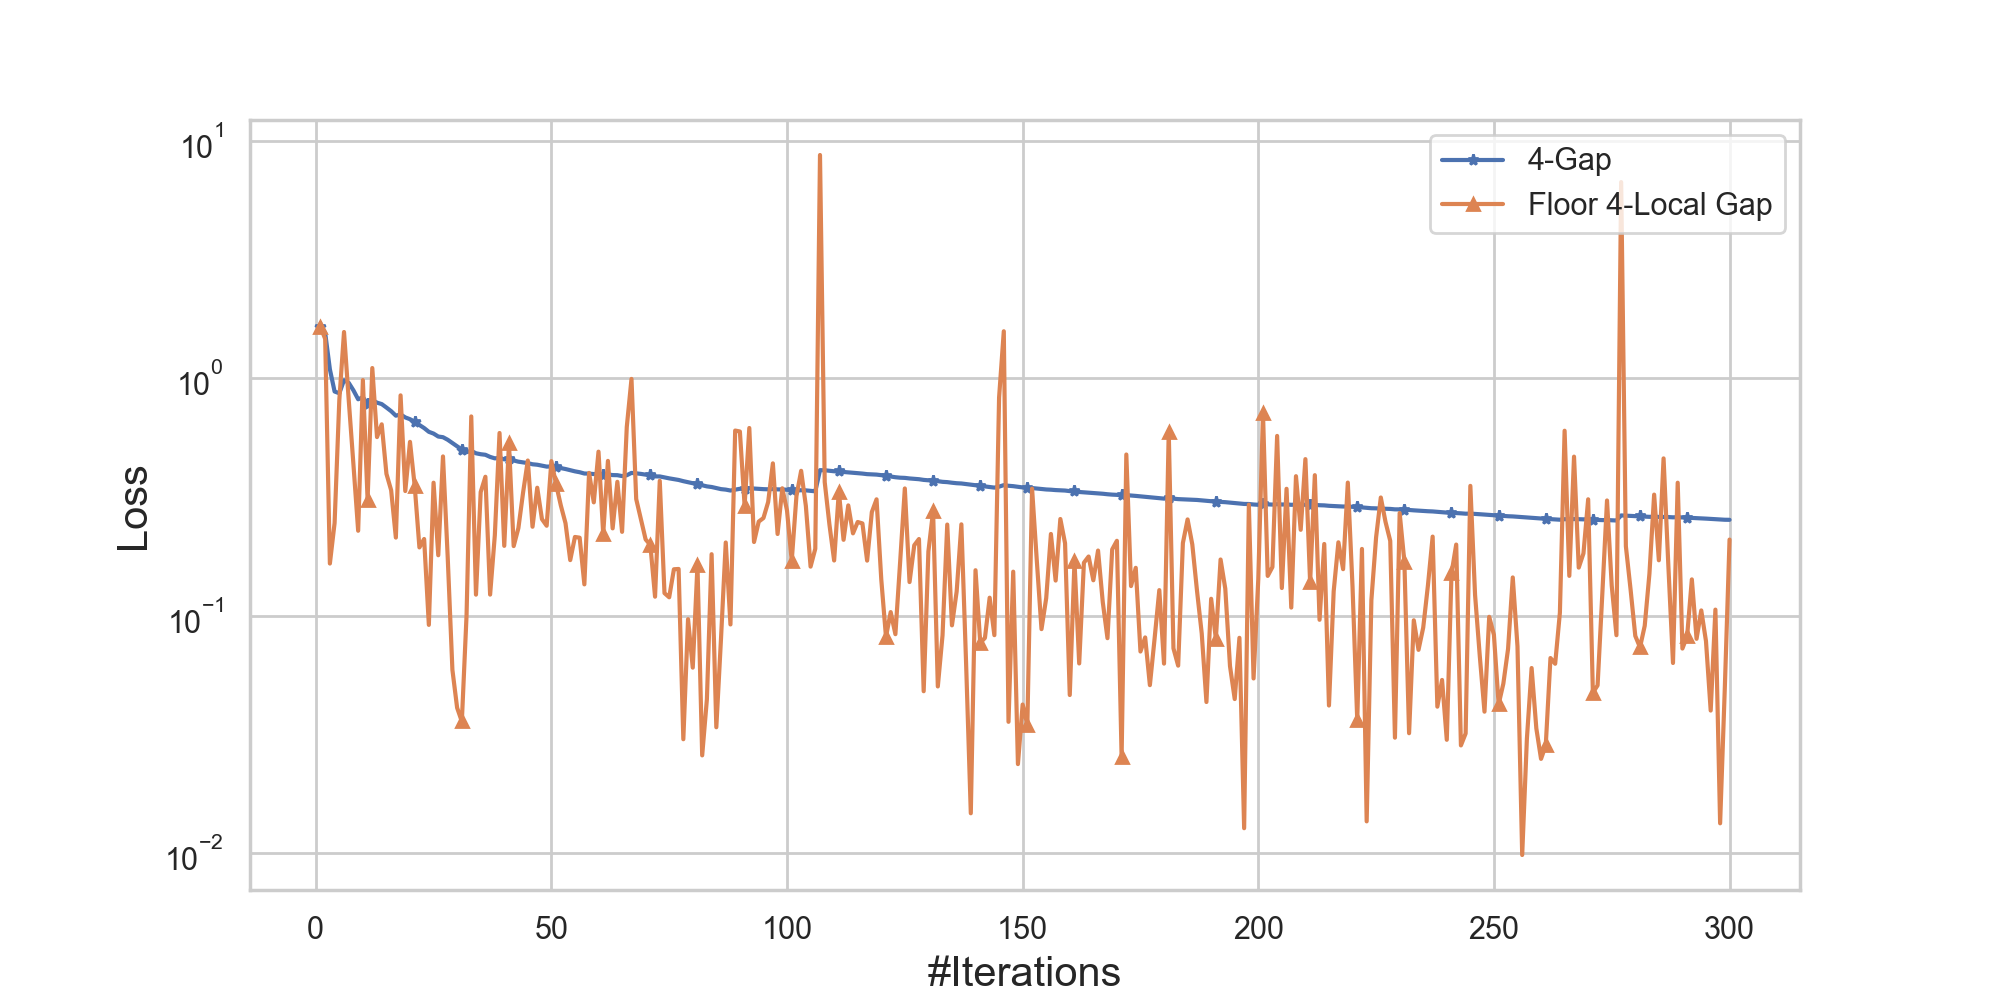
\includegraphics[width=7cm]{img/onlineGap-f4.png} }}%
%     \qquad
%      \subfloat[\centering Comparative Floor Wise Gaps   ]{{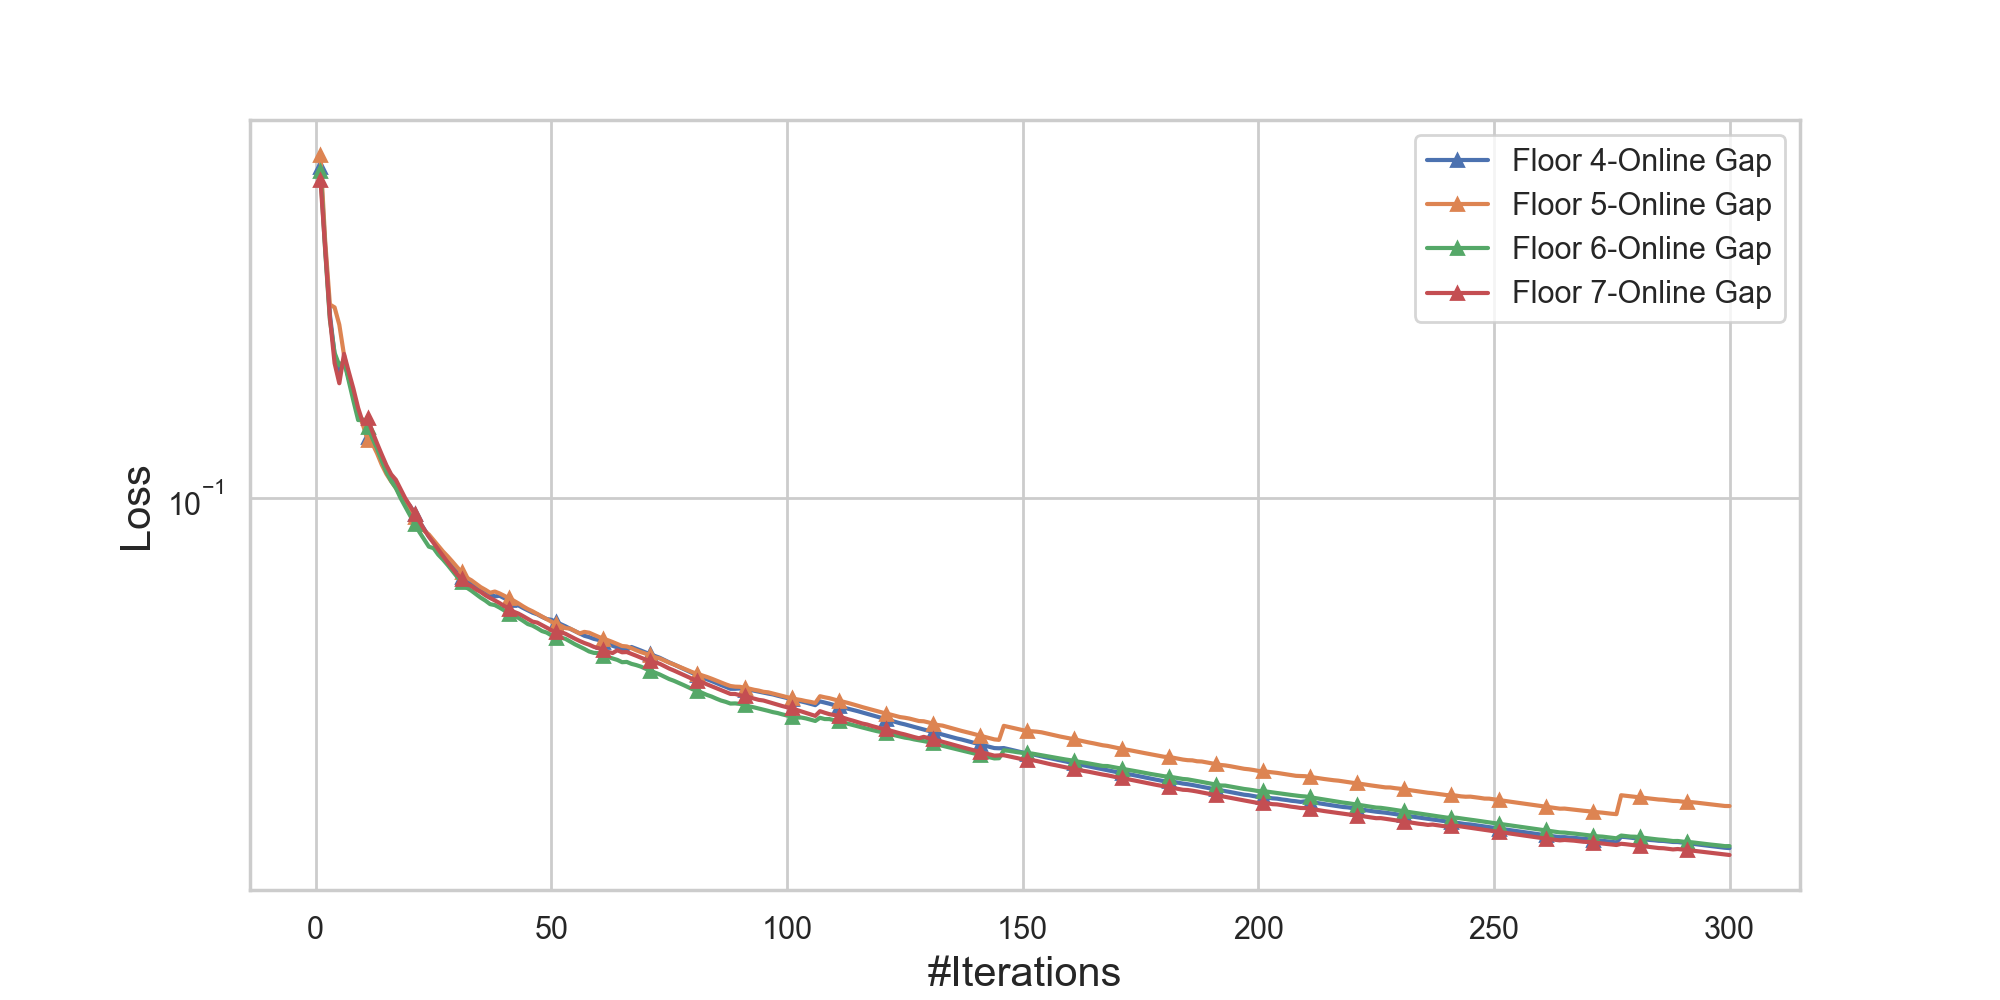
\includegraphics[width=7cm]{img/onlineGap-fall.png}}}%
%     \caption{Online Forecasting Model Quality}%
%     \label{fig:onlineGapFloorWise}%
% \end{figure}



% \begin{figure}%
%     \centering
%     \subfloat[\centering Power Variation Profile ]{{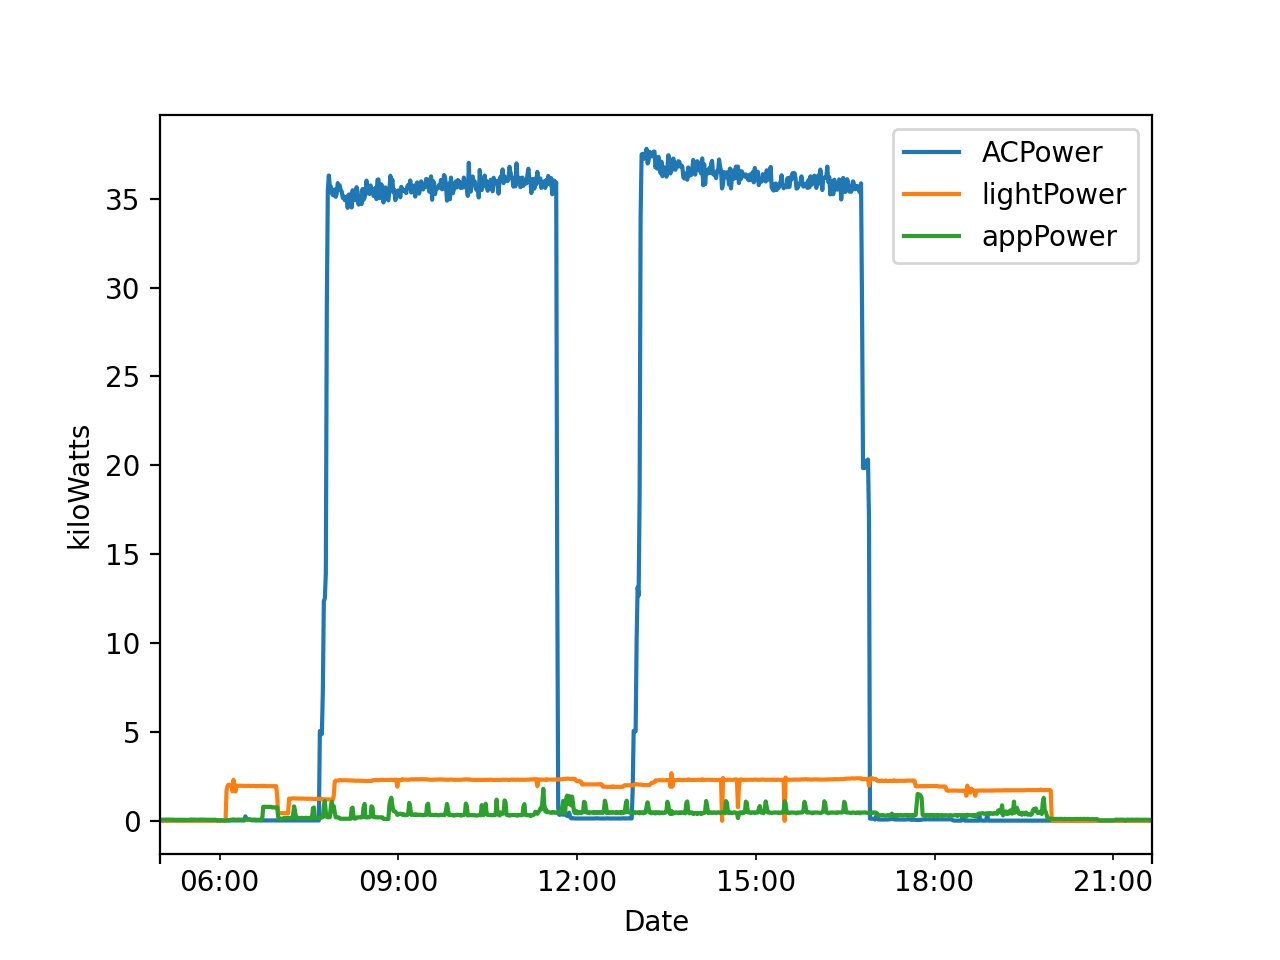
\includegraphics[width=7cm]{img/powerf7z1.png} }}%
%     \qquad
%     \subfloat[\centering Ambient Sensor Variation ]{{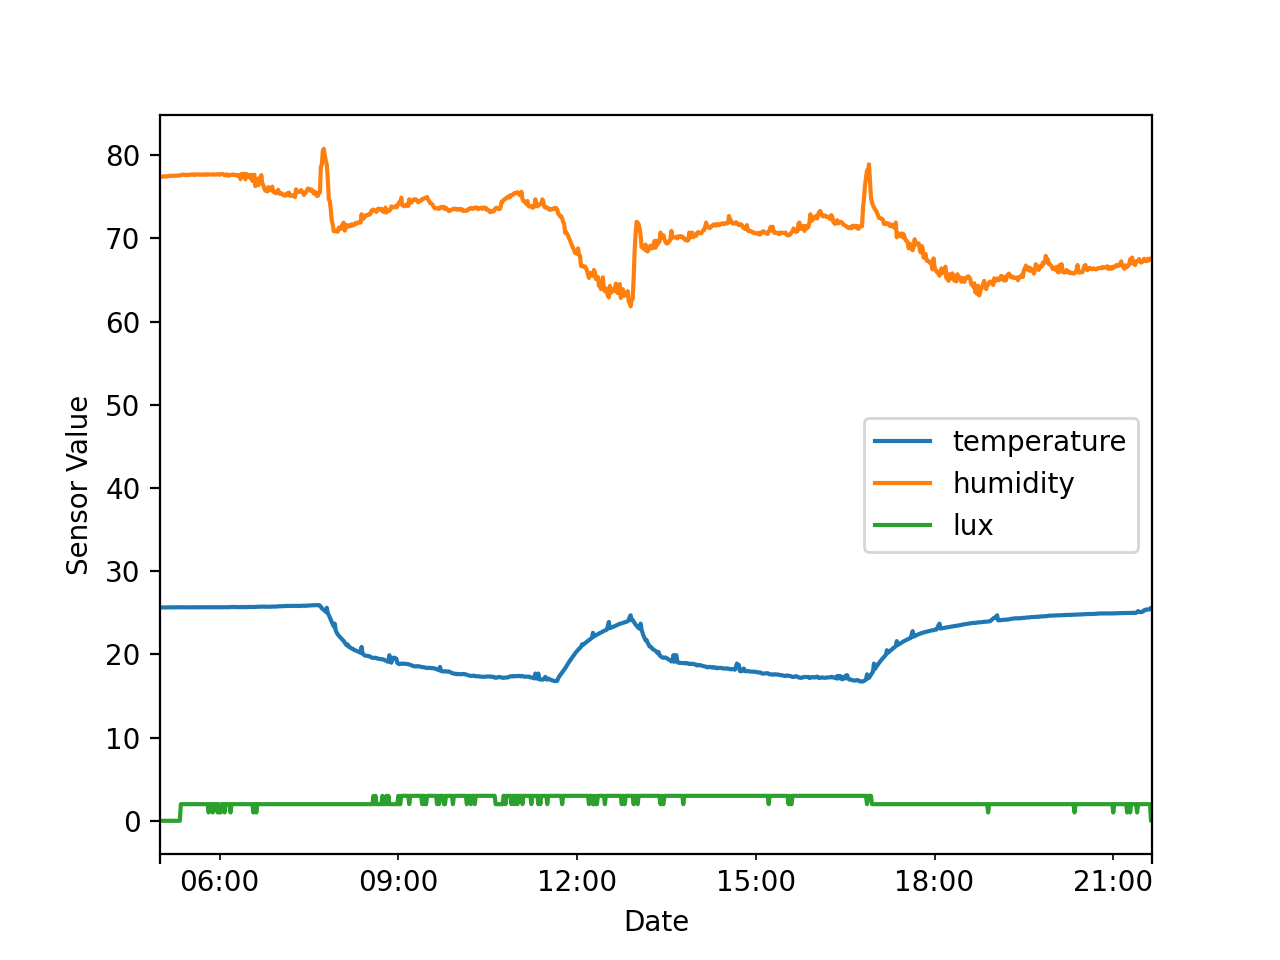
\includegraphics[width=7cm]{img/ambientf7z1.png} }}%
%     \caption{Smart Building Data Sample from a zone}%
%     \label{fig:sbdata}%
% \end{figure}
% The machine learning task for each node was one step look-ahead forecasting task at a resolution of 1 minute. 
% The setting involves online training of zonal forecasting models through knowledge sharing with other zones on the same floor. 
% The size of a look-back period quantifies the contribution of the past for a time series forecaster and is a tune able parameter. 
% We observe a reliable forecasting performance with a look-back of 13 timestamps to predict the next and will report the observations correspondingly.
% We choose to forecast 2 ambient sensor (temperature, humidity) and two power consumption (Air-conditioning,light) channels per zone.